\documentclass[12pt,a4paper]{report}
\usepackage[utf8]{inputenc}
\usepackage[T1]{fontenc}
\usepackage{lmodern}
\usepackage{microtype}
\usepackage{amsmath, amssymb, amsthm}
\usepackage{geometry}
\geometry{a4paper, margin=1in}
\usepackage{booktabs}
\usepackage{graphicx}
\usepackage{caption}
\usepackage[colorlinks=true, allcolors=blue]{hyperref}
\usepackage{natbib} 
\usepackage[UKenglish]{babel}
\usepackage{listings}
\usepackage{natbib}

\lstset{
    literate={Δ}{{$\Delta$}}1 % Render Delta as math symbol
           {→}{{$\to$}}1
           {α}{{$\alpha$}}1
           {θ}{{$\theta$}}1
           {_}{\_}1, % Fix underscores by escaping them
           showstringspaces=false,  % This is key - keeps spaces normal in strings
}
\usepackage{titlesec}

% Main chapters: big
\titleformat{\chapter}[display]
  {\normalfont\bfseries\Huge}
  {\chaptertitlename\ \thechapter}{20pt}{\Huge}
  
% === Title Page ===
\title{Portfolio Allocation Strategies}
\author{Maria Cucu}
\date{\today}

\graphicspath{{Images/}}

\begin{document}

\maketitle

\tableofcontents
\newpage

% === Chapters ===
\chapter{Summary}

Portfolio allocation remains a central problem in financial economics, bridging theory, empirical analysis, and practical decision-making. At its core, the allocation problem asks how capital should be distributed across asset classes in a way that aligns with investor objectives, risk tolerance, and time horizons. Since the seminal work of \citet{Markowitz1952}, which formalised the principles of diversification and the efficient frontier, portfolio theory has evolved into a rich field encompassing both static and dynamic methodologies. Traditional approaches such as Buy and Hold (BAH) are grounded in the Efficient Market Hypothesis \citep{Fama1970} and the belief in long-term wealth accumulation through passive exposure, while more active frameworks -- such as the Constantly Rebalanced Portfolio (CRP), momentum-based investing, and contrarian strategies -- challenge these assumptions by exploiting volatility, persistence, and overreaction in asset prices. More recently, aggregation methods, such as Cover\textquotesingle s (\citeyear{Cover1991}) universal portfolio, have sought to combine distinct allocation rules to mitigate regime-specific risks and enhance resilience.

The objective of this thesis is to conduct a comparative empirical evaluation of these approaches -- BAH, CRP, momentum, contrarian, and a hybrid aggregated strategy -- across sharply divergent market regimes. The analysis is designed to move beyond testing strategies under a single set of conditions, instead situating them within both a high-growth, innovation-driven equity environment and a stressed environment composed of persistently underperforming assets. This dual framework provides a benchmark for assessing performance in favourable conditions while simultaneously stress-testing the ability of each strategy to withstand prolonged adversity.

Each methodology reflects a distinct view of market behaviour. BAH embodies confidence in long-term efficiency and growth but exposes investors to drawdowns during crises or secular stagnation. CRP leverages mean reversion by systematically rebalancing toward fixed weights, “harvesting volatility” in oscillating markets. Momentum strategies capture the empirical tendency of winners to continue outperforming in the short to medium term \citep{Jegadeesh1993}, while contrarian strategies profit from eventual rebounds in oversold assets, assuming prices revert toward levels supported by fundamentals \citep{DeBondt1985}. The aggregated strategy introduced here combines momentum and contrarian signals, seeking to reduce the regime-specific vulnerabilities of each by dynamically reallocating between them.

A further contribution of this thesis is methodological. Performance is assessed using a dual-metric framework selected for its relevance to both investor psychology and institutional mandates. The Sharpe ratio \citep{Sharpe1966, Sharpe1994} captures risk-adjusted performance by relating excess returns to the volatility of the portfolio, offering a standardised measure of efficiency that facilitates comparison between strategies. To complement this volatility-based perspective, Maximal Drawdown \citep{MagdonIsmail2004} is employed as a path-dependent indicator of worst peak-to-trough loss. Whereas the Sharpe ratio highlights return efficiency, MDD provides a clinically relevant measure of downside risk, reflecting the practical concerns of investors focused on capital preservation during periods of market stress.

Ultimately, this thesis investigates whether resilience in portfolio management can be better achieved not solely through diversification across asset classes, but through diversification across allocation philosophies. By constructing a meta-strategy that dynamically integrates competing paradigms, it seeks to advance a more adaptive framework for portfolio construction. In doing so, the study contributes both to the theoretical literature on allocation under uncertainty and to the practical challenge of building portfolios capable of sustaining long-term growth while limiting the severity of capital erosion.

\chapter{Introduction and Literature Review}
% Insert literature review here

Portfolio allocation remains a foundational challenge in financial economics and investment management, both at an academic and a practical level. The origins of portfolio allocation theory can be traced back to the early twentieth century, but it was the formalisation by \citet{Markowitz1952} that initiated a revolution, introducing the concept of diversification and the efficient frontier. The efficient frontier represents the set of portfolios that achieve the highest possible expected return for a given level of risk, or equivalently, the lowest possible risk for a given level of expected return. Portfolios lying inside the frontier are considered suboptimal because there exists an alternative combination of assets that offers a strictly better risk–return trade-off. This framework formalised the idea that investors should not evaluate assets in isolation, but rather as components of a portfolio whose overall risk and return depend on correlations among holdings.

At its core, the allocation problem asks how to distribute capital, often across a wide array of asset classes, such as stocks, bonds, commodities, and alternatives, in a way that aligns with the goals, risk tolerance, and time frame of an investor. In mathematical terms, the allocation problem is an optimisation exercise: given estimates of asset returns, volatilities, and correlations, the investor seeks the portfolio weights that balance expected return against risk in line with their preferences. In practice, however, this problem extends beyond pure mathematics, as it requires consideration of estimation errors, changing market conditions, transaction costs, liquidity needs, and behavioural factors \citep{Campbell2002}. 

The complexity of this task has steadily increased in the face of globalised financial markets, rapid innovation in investment products, and the emergence of new risks and opportunities. In academic research, portfolio allocation is situated at the intersection of economics, probability theory, and behavioural finance, reflecting the rich interplay between quantitative modelling and the real-world decisions faced by practitioners. The policy implications of sound portfolio allocation resonate widely, influencing not only professional fund managers and institutional investors, but also individuals with long-term financial goals. Ultimately, the capital allocation decision shapes the trajectory of wealth accumulation, risk exposure, and resilience to market disruptions, making it a central problem that has inspired decades of research and debate. 

Since the foundational work by \citet{Markowitz1952}, a rich field of portfolio theory and quantitative strategy design has evolved, giving rise to multiple allocation methodologies, each built on distinct assumptions about market behaviour and investor priorities. More recently, advances in empirical finance and machine learning have opened new approaches for addressing these challenges, and have also underscored the limits of traditional models when faced with high-dimensional data and dynamic market environments \citep{Gu2020}. While these novel approaches promise more adaptive and data-driven allocation methods, they also face practical challenges, including model overfitting, sensitivity to input assumptions, and limited transparency in decision-making. As such, despite the sophistication of modern techniques, traditional strategies continue to serve as important benchmarks for both researchers and practitioners.

A traditional approach, known as Buy and Hold (BAH), is rooted in the Efficient Market Hypothesis (EMH) and the belief in long-term economic growth as reflected in asset prices \citep{Fama1970}. In this framework, investors allocate their capital according to initial constant target weights and abstain from any further trading, regardless of evolving price dynamics or new information. The implicit assumption is not that investors or models can forecast short-term price movements, but rather that markets are informationally efficient and will, over time, reward patient capital through broad economic growth and the compounding of returns. Thus, the only 'prediction' embedded in BAH is that well-diversified exposure to reliable asset classes, such as equities or government bonds \citep{Malkiel2019}, will outperform more active strategies after accounting for costs and risk over long horizons.

BAH’s appeal lies in its simplicity, lack of transaction costs, and the ability to harness the compounding effects of asset appreciation over time \citep{Bogle1999}. Nevertheless, this strategy is not without its limitations: BAH leaves investors vulnerable to severe drawdowns (extended declines from a portfolio’s peak value) during market downturns or in stagnating sectors, since it does not adapt to adverse trends or shifts in the macroeconomic environment; in the short term, price fluctuations (volatility) can result in temporary losses, while the benefits of compounding returns, including reinvested dividends, materialise only over long horizons \citep{Malkiel2019}. The success of BAH thus depends heavily on the initial asset selection and the persistence of long-term growth trends.

Cases where BAH has proven particularly effective include the postwar expansion in U.S. equities, where investors who maintained broad exposure from the 1950s through the late 1990s experienced substantial real wealth accumulation, benefitting from the compounding of returns over multiple decades \citep{Siegel1998}. The outperformance of low-cost S\&P 500 index funds relative to the overwhelming majority of actively managed funds from 1970 to 2010 further highlights BAH’s value in minimising costs and delivering compounding returns \citep{French2008}. Another prominent example came after the 2008 Global Financial Crisis, when investors who held diversified stock portfolios throughout the downturn and recovery regained losses and realised significant long-term gains by 2013 \citep{Bogle2012, Malkiel2019}. While short-term volatility during the crisis caused steep declines in portfolio values, the long-term growth trajectory of equities and the reinvestment of dividends allowed patient investors to recover and exceed pre-crisis wealth levels. This episode particularly demonstrates the resilience of the BAH strategy: although it offers no protection against temporary drawdowns, its focus on long-term market participation ensures that investors benefit from the eventual recovery and the cumulative effect of compounding returns over time.

However, there are also pronounced instances in which Buy and Hold strategies have underperformed or exposed investors to severe losses. The Japanese stock market’s experience since the late 1980s offers a striking example: investors who purchased and held the Nikkei 225 at its all-time high in December 1989, just before Japan’s asset bubble collapsed, faced decades of steep losses and incomplete recovery \citep{Campbell2001}. Sector-specific BAH approaches can be equally hazardous, as seen in the long-term decline of media and telecommunications stocks after the dot-com bubble, where many constituent firms failed to recover or even exited the market \citep{Ofek2003}. Moreover, individual stocks such as Kodak or General Motors, once blue-chip staples, provide cautionary cases where BAH led to permanent capital loss as industry disruptions rendered business models obsolete \citep{Friedman2011}. When markets or sectors experience prolonged stagnation, structural decline, or permanent obsolescence, as with Japan’s post-1989 equity market, failed sectors after the dot-com bubble, or disrupted individual firms like Kodak and General Motors, holding assets passively does not allow investors to avoid losses or capture value elsewhere. In each of these cases, BAH proved unhelpful because the strategy relies on the assumption that asset prices will recover over the long term.

Empirical evidence has demonstrated that while BAH portfolios -- such as broad-market index funds -- have outperformed a majority of actively managed funds over multiple decades, they can also experience prolonged periods of underperformance and deep losses during market crises \citep{Siegel1998, French2008}.

Responding to the inflexibility of BAH, more active strategies such as Constantly Rebalanced Portfolios (CRP) have gained traction in both theory and practice. CRP strategies, formalised by \citet{Cover1991}, maintain constant target weights through periodic rebalancing, buying and selling assets at fixed intervals to restore the original allocation. This process exploits mean-reverting behaviour in asset prices, allowing investors to sell assets that have risen relative to their targets and buy those that have fallen -- effectively ``harvesting volatility''. Mean reversion refers to the tendency of asset weights to drift around their long-term targets, and “harvesting volatility” describes how CRPs systematically profit from these oscillations by buying underweight assets and selling overweight ones, capturing gains from relative price movements even without overall market trends. Empirical studies have shown that CRP can outperform BAH, particularly in markets characterised by frequent oscillations and reversals, provided transaction costs (incurred by repeated buying and selling) remain low \citep{DeMiguel2009}.

CRP and constant-mix strategies have found strong success in several important scenarios, outperforming BAH portfolios in volatile, mean-reverting markets. During the 1973–1986 period, CRP portfolios applied to the U.S. equity-bond markets generated superior risk-adjusted returns versus BAH, as rebalancing took advantage of market volatility and mean reversion \citep{Perold1988}. Similarly, CRP strategies delivered higher risk-adjusted returns and lower drawdowns in mixed-asset portfolios (i.e., portfolios combining equities, bonds, and commodities) during the turbulent 1970s inflation era, when commodity and equity returns often moved in opposite cycles \citep{Ilmanen2011}.

However, the limitations of CRP are evident under certain persistent trends or high transaction cost environments. CRP strategies performed poorly in the U.S. stock market throughout the 1995–1999 technology-led bull market, as continual rebalancing away from outperforming tech equities led to missed long-term gains \citep{French2008}. During the roaring bull run from 2009 to 2021, when U.S. equity outperformance was unusually consistent, constant-mix approaches underperformed BAH and momentum, as they systematically cut exposure to winning assets \citep{Asness2015}. Furthermore, research shows that in real-world trading with even modest transaction costs, the potential benefits of CRP strategies are often offset or reversed; \citet{DeMiguel2009} found that accounting for trading frictions (i.e., transaction costs, bid–ask spreads, and other costs of executing trades) could fully erode the advantages of high-frequency rebalancing in both simulated and empirical backtests.

Momentum-based strategies challenge the predictions of the EMH by betting on the empirical regularity that assets with strong recent performance tend to continue outperforming in the near future. One of the most studied forms is cross-sectional equity momentum, where stocks are ranked relative to one another on the basis of past returns, and portfolios are constructed by buying recent “winners” and shorting recent “losers” \citep{Jegadeesh1993}. The foundational work by \citet{Jegadeesh1993} showed that sorting assets on past returns and investing in recent winners yields significant positive excess returns -- a finding documented across a diverse set of asset classes and geographies. The theoretical literature attributes momentum profits to various behavioural factors, such as investor herding, slow information diffusion, and the underreaction to news \citep{DeBondt1985, DeBondt1987, Barroso2015}.

Momentum’s success is supported by multiple high-profile empirical findings. First, \citet{Jegadeesh1993, Jegadeesh2001} demonstrated pronounced positive returns to cross-sectional equity momentum strategies in U.S. stocks during the 1965–1989 period, a result that has held across international equity markets as well \citep{Rouwenhorst1998}. Second, \citet{Moskowitz2012} reported consistent outperformance of trend-following momentum in diverse global markets -- including equities, commodities, currencies, and bonds -- over a century of data. Third, \citet{Barroso2015} found that risk-managed equity momentum strategies delivered attractive risk-adjusted returns and lower drawdowns during volatile market environments.

Despite these successes, momentum is vulnerable to sharp reversals. \citet{Daniel2016} showed that momentum suffered dramatic ``crashes'' during strong market recoveries, such as the 2009 post-crisis rebound, when portfolios of past winners temporarily underperformed portfolios of past losers, leading to large short-term losses. \citet{Fama1996} noted that momentum approaches can yield sustained losses during certain market turnarounds, including the Asian Financial Crisis of 1997–1998, when reversal dynamics dominated. Also, momentum strategies employed in emerging markets, such as Brazil and Turkey during episodes of rapid regulatory change and market intervention, have experienced periods of significant underperformance or even negative returns \citep{Chui2010}.

Alternatively, contrarian or anti-momentum strategies intentionally target recent losers based on the premise of mean-reverting price behaviour. Classic studies, such as \citet{DeBondt1985}, empirically documented that securities with poor past performance tend to outperform former winners over longer horizons, attributing these return reversals to market overreaction and subsequent correction. The appeal of contrarian investing lies in its ability to capitalise on sentiment-driven overshooting and subsequent realignment with fundamental value. 

Examples of successful contrarian strategies include the long-term winner-loser reversals observed in U.S. equities, where the portfolios buying the worst performers of the prior three to five years (often punished by excessive investor pessimism) outperformed portfolios of prior winners, as documented by \citet{DeBondt1985, DeBondt1987}. International markets have echoed these findings, with Japan and the U.K. displaying similar return patterns, especially during periods following dramatic market crashes: after the bursting of Japan’s late-1980s equity and real estate bubble and during the U.K.’s market turmoil following the 1973–1974 oil crisis and the 1987 crash, previously underperforming stocks tended to outperform past winners as prices gradually reverted toward levels justified by underlying fundamentals \citep{Richards1997}. Another instance of contrarian outperformance was noted following the bursting of the dot-com bubble, where previously distressed technology and internet stocks, such as software firms and early e-commerce companies, experienced significant rebounds as valuations gradually normalised \citep{Chan1996}.

Nonetheless, contrarian strategies have faced marked failures in several contexts. One risk manifests in the persistence of structural decline or disruption, such as value traps -- where companies appearing as bargains continue to underperform or fail. Recent decades have seen such effects in declining sectors like coal mining or print media, where mean reversion failed to materialise and losses deepened for contrarian investors \citep{Lakonishok1994}. The energy sector’s protracted downturn from 2014–2020 further illustrates this hazard, as early contrarian bets on oil and gas stocks led to severe drawdowns before conditions stabilised \citep{Asness2015}. Empirical backtests also reveal that contrarian approaches can suffer during persistent bull trends, notably in emerging markets such as China during the 2005–2007 rally, when previous losers continued to lag as broad uptrends persisted \citep{Chui2010}.

Given that contrarian strategies can endure extended drawdown periods and may require high portfolio turnover, successful implementation often demands patience and robust risk management, such as careful position sizing, broad diversification, and limits on losses to mitigate exposure to prolonged underperformance \citep{DeBondt1987}.

Recent advances in portfolio theory have advocated for aggregating and combining distinct strategies to achieve more robust risk-adjusted returns. Cover\textquotesingle s (\citeyear{Cover1991}) Universal Portfolios theorem presents a formal method of capital allocation across a pool of strategies or ``expert portfolios'', such that the aggregate portfolio asymptotically matches the performance of the best-in-hindsight constituent strategy \citep{Ordentlich1998}. Empirical work has confirmed the benefits of aggregation -- by dynamically allocating across momentum, contrarian, CRP, and BAH methodologies, investors can often reduce  maximal drawdowns and improve resilience against regime shifts and market anomalies \citep{Lu2025TrendFolios}.

This study contributes to the literature by undertaking a comparative empirical analysis of the aforementioned allocation strategies -- BAH, CRP, as well as aggregated approaches -- across two markedly different market regimes to evaluate their robustness. In particular, we introduce a combined Momentum + Anti-Momentum portfolio, applying Cover\textquotesingle s (\citeyear{Cover1991}) aggregation principle to reconcile these two opposing signals. This approach is justified by their complementary nature: momentum typically outperforms during persistent trends, while contrarian strategies excel during market reversals. This study also introduces a meta-strategy that aggregates BAH, CRP, and the Momentum/Contrarian hybrid within the framework of Cover\textquotesingle s (\citeyear{Cover1991}) Universal Portfolio. The approach extends the principle of diversification beyond asset classes to the level of allocation philosophies, dynamically reallocating capital across competing strategies. By doing so, it seeks to mitigate the regime dependency of individual methodologies and to construct a portfolio that adapts continuously to evolving market conditions.

The strategies will be applied to two distinct portfolios: a high-growth portfolio comprising the `Magnificent Seven'' (\texttt{AAPL}, \texttt{MSFT}, \texttt{NVDA}, \texttt{AMZN}, \texttt{META}, \texttt{GOOGL}, \texttt{TSLA}), representing dominant, innovative technology and consumer discretionary firms, and a portfolio of the worst performers (\texttt{WBD}, \texttt{PARA}, \texttt{APA}, \texttt{WBA}, \texttt{PCG}, \texttt{VTRS}, \texttt{LYB}), representing challenged stocks from sectors like energy, traditional media, and pharmaceuticals, which have faced secular decline \citep{YahooFinance2025}. A ten-year horizon (2015-2025) is selected to encapsulate a full market cycle, including a prolonged bull market and significant corrections, providing a sufficiently large dataset for robust statistical inference. Allocation and rebalancing will be performed at daily, weekly, and monthly frequencies to assess the impact of trading horizons on strategy efficacy and transaction cost sensitivity.

Critically, to capture the true economic return an investor would achieve, this study utilises adjusted closing prices, which account for corporate actions such as stock splits and, most importantly, dividend payments \citep{Bodie2023}. This methodological choice is essential for a fair comparison, as the two portfolios have starkly different dividend policies. While some ``Magnificent Seven'' constituents pay negligible dividends, the portfolio's return is overwhelmingly driven by capital growth, in stark contrast to the income-dependent ``Worst Seven'' portfolio. The ``Worst Seven'' portfolio contains several high-yielding, income-generating stocks, and ignoring dividends would systematically bias results by understating their total return and overstating their drawdowns. 

Performance will be evaluated on a total return basis through two pivotal metrics: the Sharpe ratio, to quantify risk-adjusted returns by measuring excess return per unit of volatility \citep{Sharpe1966, Sharpe1994}, and maximal drawdown (MDD) \citep{MagdonIsmail2004}, which quantifies the worst peak-to-trough loss experienced by a portfolio over a specified time frame, offering a more path-dependent, investor-centric and actionable metric than symmetrical volatility. The impact of dividends is expected to be asymmetric: for the low-yield ``Magnificent Seven'', the Sharpe ratio and drawdown figures will be largely driven by capital appreciation, while for the higher-yield ``Worst Seven'', the reinvestment of dividends should provide a cushion against capital depreciation, potentially leading to a meaningfully higher Sharpe ratio and a less severe MDD than price return alone would suggest. This dual evaluation will provide a holistic view of whether a strategy's returns are adequately compensated for their risk and how resilient they are to significant market downturns, thereby offering nuanced insights into the practical viability of each approach under contrasting economic conditions.

\chapter{Methodology}
% Insert methodology (maths, simulation setup, etc.)

This chapter presents the methodological framework for evaluating the performance of alternative portfolio allocation strategies. The analysis is organised around two core components: a theoretical foundation, which formalises the mathematical representation of portfolio growth, rebalancing mechanisms, and transaction costs; and an empirical implementation, which translates these concepts into practice through computational models that can be reproduced across diverse contexts. The overarching objective is to design, simulate, and assess the effectiveness of multiple allocation strategies under realistic market conditions, explicitly accounting for trading frictions and testing their performance across both growth-oriented and distressed asset classes.

\section{Theoretical Framework of Portfolio Allocation}
\label{sec:theory}

The investment process is modelled as a discrete sequence evolving over \( T \) trading periods. Following from \citet{Markowitz1952}, each portfolio comprises \( m \geq 1 \) assets, with closing prices at time \( t \) denoted by \( X_t^1, X_t^2, \ldots, X_t^m \geq 0 \), alongside a risk-free cash asset, assumed for simplicity to yield zero interest. The net return of asset \( i \) between periods \( t-1 \) and \( t \) is defined as:
\begin{equation}
R^i_t = \frac{X^i_t - X^i_{t-1}}{X^i_{t-1}}.
\label{eq:returns}
\end{equation}
The associated growth factor for asset \( i\) over the same time interval is \( (1 + R^i_t) = X^i_t / X^i_{t-1} \). Values greater than or equal to one represent a profit, while values below one indicate a loss. The logarithmic return, \( \log(1 + R^i_t) \), provides a convenient approximation for compounding across multiple periods. The cumulative growth of a single asset from time \( 0 \) to \( T \) is obtained by multiplying the growth factors of each period:
\begin{equation}
\frac{X_T^i}{X_0^i} = \prod_{t=1}^{T} (1 + R^i_t).
\label{eq:cumgrowth}
\end{equation}

An allocation strategy \citep{Malkiel2019} is defined by a vector \( \boldsymbol{\theta}_t = (\theta^1_t, \theta^2_t, \ldots, \theta^m_t) \) that specifies the proportion of the total portfolio value invested in each asset at the beginning of period \( t \). The strategy is restricted to long-only positions, so all weights satisfy (\( \theta^i_t \geq 0 \)). Leverage is not allowed, implying (\( \sum_{i=1}^m \theta^i_t \leq 1 \)). The remaining proportion, \( 1 - \sum_{i=1}^m \theta^i_t \), is allocated to cash. A critical assumption is that the strategy \( \boldsymbol{\theta}_t \) can depend only on information available up to time \( t-1 \), ensuring no look-ahead bias (i.e., the artificial use of future information in portfolio decisions, which would otherwise lead to overstated performance).

Given an initial capital \( V_0 \), the evolution of the portfolio value is governed by the recursive equation:
\begin{equation}
V_t = V_{t-1} \left( 1 - \sum_{i=1}^m \theta^i_{t-1} + \sum_{i=1}^m \theta^i_{t-1} \frac{X^i_t}{X^i_{t-1}} \right) = V_{t-1} \left(1 + \sum_{i=1}^m \theta^i_{t-1} R^i_t \right).
\label{eq:value_recursive}
\end{equation}
The log-value of the portfolio at terminal time \( T \) is therefore given by the sum of the log-periodic returns:
\begin{equation}
\ln V_T(\boldsymbol{\theta}) = \sum_{t=1}^{T} \ln\left(1 + \sum_{i=1}^m \theta^i_{t-1} R^i_t \right).
\label{eq:log_value}
\end{equation}

The logarithmic portfolio value is the primary metric for comparing absolute strategy performance over time, which intuitively shows compounded growth and periods of decline.

\section{Investment Strategies}
\label{sec:strategies}

The Buy-and-Hold (BAH) and Constantly Rebalanced Portfolio (CRP) are foundational strategies providing two simple but contrasting benchmarks. BAH is passive: once the initial allocation is set, no further trading takes place. Portfolio weights change automatically with asset price movements, which can lead to concentrated positions in assets that perform well. This approach avoids transaction costs but does not control diversification over time. CRP, in contrast, is active: portfolio weights are reset to fixed targets at each rebalancing step. This requires selling assets that have gained value and buying those that have lost value, which keeps the portfolio diversified but introduces continuous trading and transaction costs. Taken together, BAH and CRP highlight two extremes in portfolio management -- one that fully accepts drift with the market and another that enforces constant balance -- making them useful reference points for assessing more advanced strategies.

\subsection{Buy-and-Hold Strategy}
\label{subsec:bah}

The first benchmark strategy is the \textbf{Buy-and-Hold (BAH)} portfolio \citep{Siegel1998, Bogle1999}. It is defined by constant initial weights \( \theta^i_0 \), which determine the fraction of capital invested in each asset at time \(0\). By construction, these weights are non-negative and sum to one across all \( m \) assets, ensuring that the entire portfolio is fully allocated without leverage or leftover cash. Once established, these allocations remain unchanged throughout the investment horizon, and no transaction costs are incurred because no further trading takes place.

Its terminal value is given by:
\begin{equation}
V_T = \left(1 - \sum_{i=1}^m \theta^i_0 \right) + \sum_{i=1}^m \theta^i_0 \frac{X^i_T}{X^i_0}.
\label{eq:bah_value}
\end{equation}
In practice, while the quantity of each asset purchased remains constant, the proportion of wealth in each asset, denoted by \( \theta^i_t \), changes over time. This drift is caused by the relative price movements of the assets. For example, if one asset grows faster than the others, it will gradually represent a larger share of the portfolio. 

For a uniform BAH portfolio with equal initial allocation (\( \theta^i_0 = 1/m \)), each asset receives the same fraction of the starting wealth, and the weights explicitly sum to one. The dynamic weight at time \( t-1 \) is expressed as:
\begin{equation}
\theta^i_{t-1} = \frac{ X^i_{t-1} / X^i_0 }{ \sum_{j=1}^m X^j_{t-1} / X^j_0 }.
\label{eq:bah_dynamic_weight}
\end{equation}

Thus, the Buy-and-Hold strategy reflects a passive approach where weights evolve naturally with asset price dynamics, without any further trading after the initial investment.

\subsection{Constantly Rebalanced Strategy}
\label{subsec:crp}
The second benchmark is the \textbf{Constantly Rebalanced Portfolio (CRP)} \citep{Cover1991}. Unlike BAH, this strategy maintains fixed target weights, \( \theta^i_t = 1/m \) for an equally weighted CRP. After each period, the portfolio is rebalanced to restore the target proportions, and each rebalancing incurs transaction costs proportional to the traded amount (Equation \ref{eq:net_value}).


Rebalancing requires selling a fraction of assets that have increased in value and reinvesting in those that have fallen behind. As a result, CRP systematically transfers capital from recent winners to recent losers.

The portfolio value evolves according to:
\begin{equation}
V_t = V_{t-1} \left( \sum_{i=1}^m \frac{1}{m} \frac{X^i_t}{X^i_{t-1}} \right) = \prod_{s=1}^{t} \left(1 + \sum_{i=1}^m \frac{1}{m} R^i_s \right),
\label{eq:crp_value}
\end{equation}
with transaction costs subtracted at each rebalancing step.

This mechanism enforces mean-reversion across assets and ensures that portfolio weights remain stable through time. In contrast to BAH, which drifts with market trends, CRP demands continuous rebalancing and trading activity and explicitly accounts for the costs of trading.

\subsection{Specification of Dynamic Strategies}
\label{subsec:dynamics}

Beyond the static BAH and CRP benchmarks, dynamic strategies are formulated based on price momentum \citep{Jegadeesh1993, DeBondt1985}. In this context, momentum refers to the empirical tendency of assets that have performed well in the recent past to continue outperforming in the near future, while recent underperformers are more likely to lag. This effect is typically strongest over medium-term horizons (e.g., 6 to 12 months) and measured by ranking assets according to their past returns and adjusting portfolio weights accordingly. 

In this study, momentum signals are constructed using a lookback window of one year, consistent with empirical findings on momentum persistence. To align with the different rebalancing frequencies considered, the window is expressed in three equivalent forms: \( L = 252 \) trading days for daily rebalancing, \( L = 52 \) weeks for weekly rebalancing, and \( L = 12 \) months for monthly rebalancing. 

For each asset \( i \), the rolling maximum and minimum prices over the lookback window \([t-L, t]\) are calculated:
\begin{equation}
(X^*)^i(t-L, t) = \max_{r \in [t-L, t]} X^i(r), \quad (X_*)^i(t-L, t) = \min_{r \in [t-L, t]} X^i(r).
\label{eq:roll_max_min}
\end{equation}

These quantities establish the relative ``range'' of the asset’s price over the past \( L \) periods. The rolling maximum \((X^*)^i\) captures the highest price observed, while the rolling minimum \((X_*)^i\) captures the lowest. Together, they define the price interval against which the current price can be scaled.

Two opposing signals are then generated. The \textbf{momentum strategy} measures how close the current price \( X^i(t) \) is to its rolling maximum:
\begin{equation}
\theta^{(i)}_{\text{mom}}(t) = \frac{ X^i(t) - (X_*)^i(t-L, t) }{ (X^*)^i(t-L, t) - (X_*)^i(t-L, t) }.
\label{eq:momentum}
\end{equation}

Here, the numerator \( X^i(t) - (X_*)^i(t-L, t) \) expresses how far today’s price is above the rolling minimum, while the denominator \( (X^*)^i(t-L, t) - (X_*)^i(t-L, t) \) normalises this distance by the total price range over the window. Thus, if the current price is close to the maximum, the ratio is near 1, and if it is near the minimum, the ratio is close to 0. In effect, the strategy assigns greater weight to assets trading near their recent highs, on the assumption that they are likely to continue trending upward. For momentum, asset weights are proportional to the distance above their rolling minimum, capturing the idea that assets near recent highs are more likely to continue trending upward.

Conversely, the \textbf{anti-momentum (or mean-reversion) strategy} captures the distance from the rolling maximum:
\begin{equation}
\theta^{(i)}_{\text{anti}}(t) = \frac{ (X^*)^i(t-L, t) - X^i(t) }{ (X^*)^i(t-L, t) - (X_*)^i(t-L, t) }.
\label{eq:anti_momentum}
\end{equation}

Here, the numerator \( (X^*)^i(t-L, t) - X^i(t) \) measures how far today’s price has fallen below the rolling maximum, while the denominator again normalises by the full price range. If the asset is trading near its low, the ratio approaches 1, meaning the strategy assigns a large weight to the expectation of a rebound. If the price is at or near the maximum, the ratio approaches 0. Thus, the anti-momentum weights are proportional to the distance below the rolling maximum, reflecting the expectation that assets trading far from their peaks may revert toward their recent highs.

The vectors for each single-asset strategy are valid portfolio weights as they are non-negative and sum to one. This ensures that all available capital is allocated across the assets without leverage or short-selling, and that the portfolio value is properly normalised at each point in time. The same requirement applies to BAH, CRP, and other benchmark strategies introduced earlier. In both cases, the division by the price range ensures that signals are comparable across assets, regardless of differences in scale or volatility.

The momentum and anti-momentum strategies are constructed in a parallel manner using rolling price information over a specified lookback window. In both strategies, the raw signals are normalised at each time step so that the weights are non-negative and sum to one across all assets, ensuring full capital allocation. This produces dynamically adaptive portfolios that continuously adjust exposure to each asset based on relative performance over the past \( L \) periods, with daily, weekly, or monthly rebalancing frequencies depending on the chosen horizon. 

Transaction costs are explicitly incorporated when adjusting positions, and portfolio growth is computed iteratively, accounting for both returns and the costs of rebalancing. These two strategies are then further aggregated into a final combined Momentum + Anti-Momentum strategy, using the capital-weighted aggregation method (Equation \ref{eq:aggregated_weights}). This hierarchical aggregation creates a complex, adaptive strategy that dynamically balances between trend-following and contrarian impulses based on their recent performance.

\section{Strategy Aggregation}
\label{sec:aggregation}

The project explores the aggregation of multiple individual strategies \citep{Cover1991}. The idea is to combine the strengths of individual allocation rules while reducing their weaknesses. If \( K \) strategies with portfolio values \( V_t^{(k)} \) and weight vectors \( \boldsymbol{\theta}_t^{(k)} \) are to be combined, the aggregated strategy \( \widehat{\boldsymbol{\theta}}_t \) is formed by a capital-weighted average:
\begin{equation}
\widehat{\boldsymbol{\theta}}_t = \frac{ \sum_{k=1}^{K} \boldsymbol{\theta}_t^{(k)} \cdot V_t^{(k)} }{ \sum_{k=1}^{K} V_t^{(k)} }.
\label{eq:aggregated_weights}
\end{equation}
The value of this new aggregated portfolio is simply the average of the constituent values:
\begin{equation}
\widehat{V}_t = \frac{1}{K} \sum_{k=1}^{K} V_t^{(k)}.
\label{eq:aggregated_value}
\end{equation}
This mechanism allows for the creation of hierarchical portfolios, such as the Momentum + Anti-Momentum portfolio, and an aggregate of BAH, CRP, and momentum/contrarian strategies, which is then treated as a standalone strategy for further analysis and benchmarking.

\section{Modelling Transaction Costs}
\label{sec:transaction_costs}

A realistic evaluation of portfolio strategies must incorporate the frictions associated with trading. In financial markets, these costs arise from multiple sources, including bid–ask spreads, brokerage fees, and market impact \citep{DeMiguel2009}. Even when simplified, transaction costs can have a significant cumulative effect, particularly for high-turnover strategies like the CRP.

A cost is applied to every trade in each asset. The change in capital allocated to asset \( i \) at time \( t \) is calculated as:
\begin{equation}
\Delta^i_t = \theta^i_t V_t - \theta^i_{t-1} V_{t-1} \frac{X^i_t}{X^i_{t-1}}.
\label{eq:traded_amount}
\end{equation}
If \( \Delta^i_t > 0 \) the position in asset \( i \) is increased; if \( \Delta^i_t < 0 \), it is reduced. The transaction cost is the maximum of two terms: a proportional fee equal to (0.001\%) of the trade's absolute value or a fixed minimum fee of one currency unit. Costs apply only if a trade occurs (\( |\Delta^i_t| > 0 \)). The cost at time \( t \) is therefore:
\begin{equation}
C_t = \sum_{i=1}^{m} \left( 0.001 \cdot |\Delta^i_t| \lor 1 \right) \cdot \mathbb{I}_{\{ |\Delta^i_t| > 0 \}}.
\label{eq:transaction_cost}
\end{equation}
Cumulative costs over the investment horizon are then \( C_T(\boldsymbol{\theta}) = \sum_{t=1}^{T} C_t \), so that the net terminal wealth is:
\begin{equation}
V^{\text{net}}_T(\boldsymbol{\theta}) = V_T(\boldsymbol{\theta}) - C_T(\boldsymbol{\theta}).
\label{eq:net_value}
\end{equation}
This cost structure explicitly penalises high-turnover strategies like CRP and momentum, while the BAH strategy, after the initial purchase, incurs no costs. Without this adjustment, results risk overstating performance and misleading conclusions about relative efficiency.

\section{Benchmarking and Performance Metrics}
\label{sec:benchmarking}

The performance of all strategies is evaluated against a passive market index benchmark. This benchmark is constructed as an equi-weighted portfolio of the assets at their initial weights, with no subsequent rebalancing or cost deductions:
\begin{equation}
\text{V}_t = \frac{ \sum_{i=1}^m X^i_t }{ \sum_{i=1}^m X^i_0 }.
\label{eq:market_index}
\end{equation}
This provides a neutral baseline reflecting the general price movement of the entire asset universe.

To evaluate performance robustly, two complementary metrics are employed to supplement the analysis of the logarithmic portfolio value, each capturing a distinct dimension of risk and return.

The \textbf{Sharpe ratio} \citep{Sharpe1994} is calculated to evaluate risk-adjusted returns. It measures the excess return per unit of risk (standard deviation), providing a canonical gauge of whether a strategy's returns are adequate compensation for its volatility. Formally, it is defined as:
\begin{equation}
    \text{Sharpe} = \frac{ \mathbb{E}[R_p - R_f] }{ \sigma_{R_p - R_f} },
\end{equation}
where \(R_p\) is the portfolio return, \(R_f\) is the risk-free rate, and \(\sigma\) is the standard deviation of the excess return. A higher Sharpe ratio indicates a more efficient allocation of risk. A Sharpe ratio below 0 signals the portfolio is underperforming the risk-free rate and taking uncompensated risk, around 0 indicates minimal reward for risk, 0 to 1 reflects modest risk-adjusted returns, 1 to 2 signals solid performance, and above 2 marks exceptional efficiency in generating returns per unit of risk.

Complementing this, the \textbf{Maximal Drawdown (MDD)} \citep{MagdonIsmail2004} is calculated to evaluate tail risk and capital preservation. It quantifies the worst peak-to-trough decline in the portfolio's value before a new peak is achieved:
\begin{equation}
\text{MDD} = \max_{\tau \in (0,T)} \left[ \frac{ \max_{s \in (0,\tau)} V_s - V_\tau }{ \max_{s \in (0,\tau)} V_s } \right].
\label{eq:mdd}
\end{equation}
A larger (absolute) magnitude value of the peak-to-trough return would correspond to a larger, and therefore worse, MDD. Measured in percentages, MDD indicates the largest historical loss an investor would have experienced: values below 10\% signal minor, losses; 10–30\% reflects moderate drawdowns typical of active strategies; 30–50\% indicates severe losses that could trigger investor concern; 50–100\% shows extreme risk with substantial capital erosion; and above 100\% implies total or leveraged losses exceeding the initial investment, highlighting catastrophic failure. This metric is a crucial gauge of strategy risk and potential investor discomfort, as it captures the worst-case historical loss and directly tests a strategy's resilience during stressful market conditions, a key aim of this study.

This dual-metric framework provides a holistic view: the Sharpe ratio assesses performance under typical market volatility, while the MDD specifically stress-tests the strategy against the most severe adverse movements, addressing the critical concern of capital erosion.

\section{Empirical Implementation and Data Processing}
\label{sec:implementation}

The models are implemented in Python using standard scientific libraries: NumPy for numerical operations, Pandas for data handling, Matplotlib for visualisation, and yFinance for price data. The dataset consists of adjusted daily closing prices over a 10-year horizon, obtained via the Yahoo Finance API. Adjusted prices are used to account for dividends and stock splits, ensuring the analysis accurately reflects total returns rather than price appreciation alone.

A critical aspect of this study is evaluating the sensitivity of each allocation strategy to rebalancing frequency. Consequently, the strategies are implemented and tested on data resampled to daily, weekly, and monthly intervals. This multi-horizon approach allows for a rigorous examination of core performance questions: whether the benefits of frequent rebalancing (e.g., better capturing short-term trends for momentum or more precise volatility harvesting for CRP) are offset by increased transaction costs, and whether longer-term strategies (e.g., BAH) are indeed less sensitive to such granularity. This analysis provides crucial insights into the practical trade-offs between theoretical performance and implementable strategy design.

Two asset universes are analysed to test robustness. 
The first, the ``Magnificent Seven'', includes leading technology stocks 
(\texttt{AAPL}, \texttt{MSFT}, \texttt{NVDA}, \texttt{AMZN}, \texttt{META}, \texttt{GOOGL}, \texttt{TSLA}). 
The second, the ``Weakest Seven'', includes underperforming S\&P 500 firms 
(\texttt{WBD}, \texttt{PARA}, \texttt{APA}, \texttt{WBA}, \texttt{PCG}, \texttt{VTRS}, \texttt{LYB}), 
representing adverse market conditions.

All portfolios are initialised with a nominal value \( V_0 = 10,000 \). Each asset's price series is normalised by its initial price \( X^i_0 \) to convert absolute prices into cumulative growth factors, ensuring comparability across assets with different price scales. Weekly returns \( R^i_t \) are computed from these normalised series. Finally, the data are cleaned by removing missing values to maintain alignment across all assets in each universe.

\section{Numerical Robustness and Implementation Safeguards}
\label{sec:robustness}

The simulation code incorporates several safeguards to ensure numerical stability and robustness. These include explicit checks to prevent division by zero during normalisation and score calculations, the handling of NaN values that may arise during the initial rolling window period, and an initialisation protocol where momentum-based strategies remain flat (100\% cash) until each lookback window is fully populated with data. This prevents the generation of spurious signals from insufficient data. Finally, all portfolio values are plotted on a logarithmic scale, which not only linearises compounded returns but also facilitates comparison across portfolios of different magnitudes. This choice avoids distortion from exponential growth effects and is consistent with common practice in financial econometrics. The example code needed to compute the weekly rebalancing can be found in \textbf{Appendix B}.

\chapter{Results}

This section reports the empirical outcomes for the four portfolio strategies: Buy-and-Hold (BAH), Constantly Rebalanced Portfolio (CRP), a combined Momentum and Anti-Momentum strategy (M+AM), and an Aggregated strategy incorporating all three. Results were computed at three allocation frequencies (daily, weekly, and monthly), but only the weekly results are presented in this chapter. The daily allocation produced unstable outcomes, particularly for the CRP strategy, which failed due to excessive trading activity and transaction costs. The monthly allocation, while computationally valid, generated equity curves that appeared excessively jagged across all strategies. Such jaggedness indicates a mismatch between the rebalancing horizon and the underlying asset dynamics: too infrequent rebalancing failed to capture intermediate market trends, and the resulting portfolios oscillated sharply between gains and losses without establishing a stable trajectory. To avoid distracting from the main analysis, the daily and monthly results are documented separately in \textbf{Appendix A}. The weekly allocation thus provides the clearest picture of strategic performance, balancing responsiveness with stability.  

Performance is assessed across two contrasting asset universes, using compounded growth (shown on a logarithmic scale), Maximal Drawdown (MDD), and Sharpe ratios as key metrics. The results highlight how strategy performance depends strongly on market regime and demonstrate the stabilising effect of diversification.

\section{Performance in a High-Growth Regime: The ``Magnificent Seven''}

Figure~\ref{fig:best_log} shows the performance of all strategies applied to the high-growth ``Magnificent Seven'' universe. The logarithmic scale illustrates compounded growth and relative drawdowns.

\begin{figure}[htbp]
    \centering
    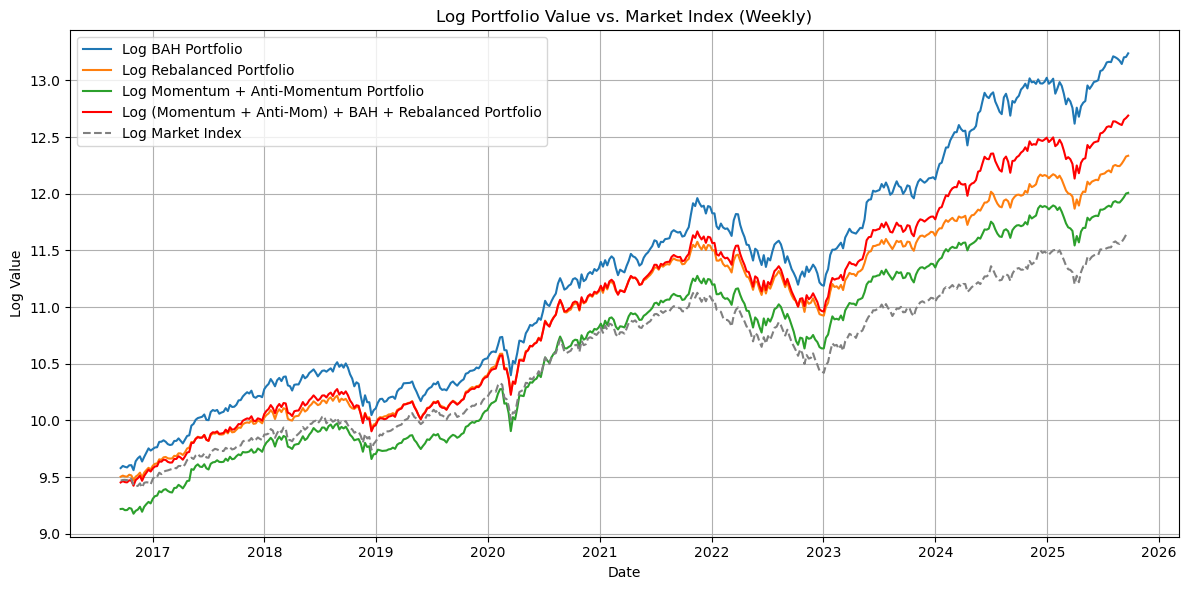
\includegraphics[width=0.95\textwidth]{best_weekly_log_values.png}
    \caption{Logarithmic portfolio value evolution for the ``Magnificent Seven'' universe (2015 -- 2025). The BAH strategy dominates in absolute performance, while the Aggregated strategy provides a smoother growth path with smaller drawdowns.}
    \label{fig:best_log}
\end{figure}

The BAH strategy delivered the strongest benchmark performance, largely driven by the sustained growth of very large technology companies. By maintaining investments in the best-performing stocks without selling, the strategy allowed gains to accumulate over time, ultimately reaching the highest terminal value by 2025. However, this strong performance came with considerable ups and downs, including steep interim losses during the 2020 COVID market crash and the 2022 inflation-driven selloff. As a result, the strategy’s risk-return profile can be described as “high risk, high reward.”  

The CRP strategy delivered slightly weaker overall performance. By systematically adjusting allocations, it smoothed the portfolio’s trajectory during periods of high volatility. However, this approach came at a cost during extended periods when certain stocks continued to rise steadily, as selling top-performing positions and increasing exposure to underperforming ones limited the compounding of gains over time. This highlights a classic drawback of contrarian rebalancing in strongly trending markets: by betting on prices returning to their historical averages, the strategy often sacrifices the benefits of momentum-driven growth.

The M+AM portfolio lagged both benchmarks. Its momentum component was able to capture some upward trends in winning stocks, but the contrarian anti-momentum positions often offset these gains by reducing exposure to high-performing assets at critical moments. This effect, combined with the higher turnover required to maintain both momentum and contrarian positions, eroded its overall risk-adjusted performance. In essence, the strategy struggled to fully participate in the persistent upward trajectory of the ``Magnificent Seven'', leaving it less competitive than either the Buy-and-Hold or the CRP during a prolonged bull market.

The Aggregated portfolio, by contrast, achieved a balanced middle ground. While it did not match the absolute growth of the Buy-and-Hold strategy, it consistently outperformed both the CRP and the M + AM approach following 2020. By dynamically reallocating capital across the three component strategies, it captured favourable returns while mitigating losses during volatile periods. The resulting smoother equity curve illustrates its appeal as a “universal” strategy: although it rarely produces the highest returns in any single period, it consistently avoids being the weakest performer, offering resilience and stability across a wide range of market conditions.

\begin{table}[h!]
\centering
\caption{Maximal Drawdowns (MDD) for the ``Magnificent Seven'' Universe}
\label{tab:mdd_best}
\begin{tabular}{lc}
\toprule
\textbf{Strategy} & \textbf{Max Drawdown} \\
\midrule
Buy-and-Hold (BAH) & -53.87\% \\
Constantly Rebalanced Portfolio (CRP) & -47.88\% \\
Momentum + Anti-Momentum (M+AM) & -47.32\% \\
Aggregated Strategy & -50.69\% \\
\textbf{Market Index} & \textbf{-50.65}\% \\
\bottomrule
\end{tabular}
\end{table}

The drawdown analysis in Table~\ref{tab:mdd_best} illustrates the trade-offs among the strategies. BAH experienced the deepest decline, nearly -54\%, reflecting its full exposure to market shocks. Both the CRP and the Momentum + Anti-Momentum strategies limited losses by roughly 6--7 percentage points. The Aggregated strategy fell in between, offering some downside protection relative to BAH while still tracking close to the market index. 

\begin{table}[h!]
\centering
\caption{Sharpe Ratios for the ``Magnificent Seven'' Universe}
\label{tab:sharpe_best}
\begin{tabular}{lc}
\toprule
\textbf{Strategy} & \textbf{Sharpe Ratio} \\
\midrule
Buy-and-Hold (BAH) & 1.35 \\
Constantly Rebalanced Portfolio (CRP) & 1.31 \\
Momentum + Anti-Momentum (M+AM) & 1.20 \\
Aggregated Strategy & 1.33 \\
\textbf{Market Index} & \textbf{1.09} \\
\bottomrule
\end{tabular}
\end{table}

The Sharpe ratios in Table~\ref{tab:sharpe_best} highlight why BAH dominated in this regime: its 1.35 ratio indicates the most efficient risk-adjusted performance. CRP and the Aggregated portfolio achieved similar values (1.31 and 1.33), showing that rebalancing and diversification provided some downside protection without significantly compromising efficiency. By contrast, M+AM lagged with a ratio of 1.20, reflecting weaker returns relative to risk. All strategies, however, comfortably outperformed the market index (1.09), emphasising the structural advantage of rule-based allocation in a strongly trending environment. 

\section{Stress Testing in a Secular Decline: The ``Weakest Seven''}

Figure~\ref{fig:worst_log} shows the performance of all strategies in the ``Weakest Seven'' universe. This setting, characterised by persistent declines and high volatility, provides a strong test of robustness.

\begin{figure}[htbp]
    \centering
    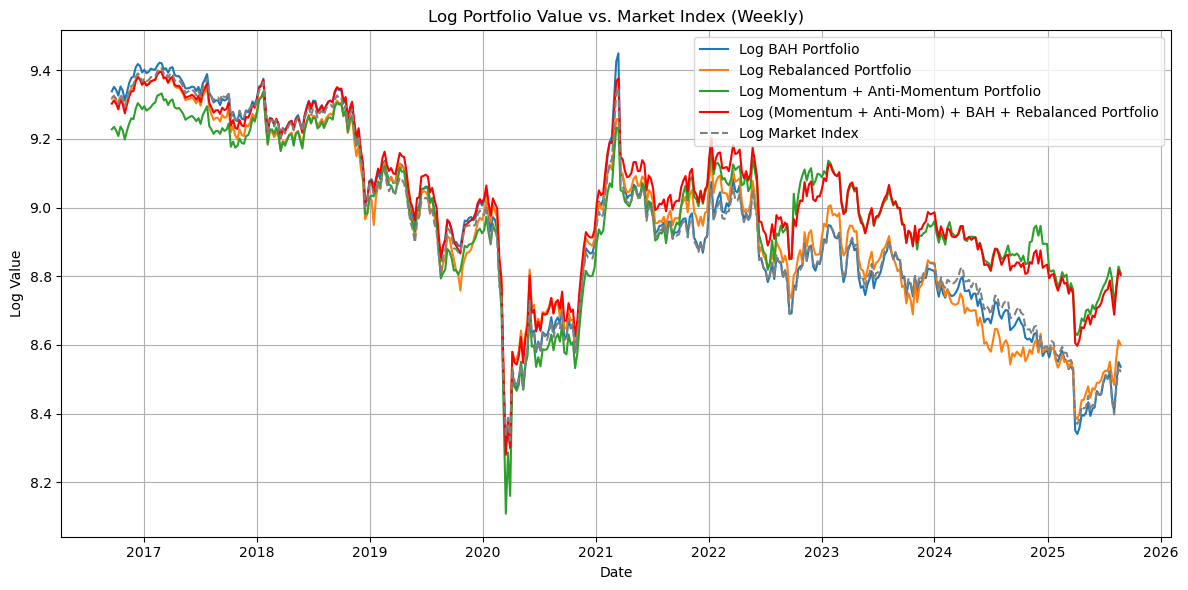
\includegraphics[width=0.95\textwidth]{worst_weekly_log_values.png}
    \caption{Logarithmic portfolio value evolution for the ``Weakest Seven'' universe (2015--2025). None of the strategies escapes large losses, but M+AM and the Aggregated strategy show relative resilience in risk-adjusted terms.}
    \label{fig:worst_log}
\end{figure}

The BAH strategy experienced a continuous decline in portfolio value, reflecting its unchanging exposure to consistently underperforming assets. The CRP offered minimal improvement, as its contrarian rebalancing into declining positions amplified losses, making its performance largely indistinguishable from BAH.

The M+AM strategy presented a mixed performance. While it endured more pronounced fluctuations and the largest single drawdown, it occasionally outperformed BAH and CRP, particularly mid-decade. This indicates that its momentum component sometimes avoided the weakest assets, although the anti-momentum positions often worked against potential recoveries. Overall, it recorded the highest Sharpe ratio in this universe, though it remained close to zero, reflecting the challenging market conditions.

The Aggregated portfolio again provided relative stability. By blending exposures, it ended above BAH and CRP by the end of the sample period, though still unable to avoid large overall losses. Its flexible approach meant it was never the top performer, but it was consistently more resilient and less vulnerable than any single strategy on its own.

\begin{table}[h!]
\centering
\caption{Maximal Drawdowns (MDD) for the ``Weakest Seven'' Universe}
\label{tab:mdd_worst}
\begin{tabular}{lc}
\toprule
\textbf{Strategy} & \textbf{Max Drawdown} \\
\midrule
Buy-and-Hold (BAH) & -67.48\% \\
Constantly Rebalanced Portfolio (CRP) & -66.56\% \\
Momentum + Anti-Momentum (M+AM) & -70.71\% \\
Aggregated Strategy & -67.18\% \\
\textbf{Market Index} & \textbf{-66.18}\% \\
\bottomrule
\end{tabular}
\end{table}

As Table~\ref{tab:mdd_worst} shows, all strategies suffered catastrophic losses in this environment. The M+AM strategy experienced the worst drawdown (-70.7\%), confirming its vulnerability to extended declines. BAH, CRP, and the Aggregated portfolio clustered near -66 to -67\%, roughly in line with the market index. The relative ordering reveals little downside protection in secular bear markets.  

\begin{table}[h!]
\centering
\caption{Sharpe Ratios for the ``Weakest Seven'' Universe}
\label{tab:sharpe_worst}
\begin{tabular}{lc}
\toprule
\textbf{Strategy} & \textbf{Sharpe Ratio} \\
\midrule
Buy-and-Hold (BAH) & -0.08 \\
Constantly Rebalanced Portfolio (CRP) & -0.07 \\
Momentum + Anti-Momentum (M+AM) & 0.03 \\
Aggregated Strategy & 0.01 \\
\textbf{Market Index} & \textbf{-0.11} \\
\bottomrule
\end{tabular}
\end{table}

The Sharpe ratios in Table~\ref{tab:sharpe_worst} provide further nuance. BAH and CRP both posted slightly negative Sharpe values (-0.08 and -0.07), indicating weak returns for the risks carried inherently. The market index was worse at -0.11, confirming that passive exposure was particularly unattractive. By contrast, M+AM managed a marginally positive Sharpe (0.03), while the Aggregated portfolio held near zero (0.01). Although small in magnitude, these results suggest that adaptive or momentum-based elements offered relative resilience compared to static allocations.  

\section{Visual Analysis of Portfolio Composition}

Further insight can be drawn from Figure~\ref{fig:weights_best}, which decomposes the evolution of the BAH and M+AM strategies for the ``Magnificent Seven'' universe. The upper panel, showing normalised asset prices ($X_t/X_0$), highlights the exceptional growth of a few dominant firms -- most notably \texttt{NVDA} -- relative to their peers. This divergence drives much of the portfolio dynamics observed in the subsequent plots. 

The middle panel shows the implicit value-weighted allocations of the BAH portfolio. As NVDA’s price appreciation outpaced all others, its portfolio weight expanded steadily to nearly 70\% of the portfolio, while the relative shares of the other constituents shrank. This illustrates both the strength and weakness of BAH: it fully captures compounding in the top performer but leaves the investor heavily concentrated and therefore exposed if the leader suffers a sharp reversal. 

The bottom panel presents the allocation dynamics of the M+AM strategy. Unlike BAH, it actively redistributes capital across assets, with weights shifting frequently as momentum and anti-momentum signals evolve. Periods of heightened volatility, such as 2022–2023, show sharp reallocations and even temporary concentration in single names when they exhibited relative strength. During volatile episodes, such as 2022–2023, the reallocations are especially sharp, sometimes concentrating heavily in one or two assets that temporarily exhibit relative strength. While such turnover generates trading costs, it also highlights the strategy’s adaptability -- allowing it to capture new leaders while reducing exposure to stocks entering decline. Overall, this visualisation highlights the structural difference between passive concentration in BAH and the adaptive, signal-driven reallocations in M+AM.

\begin{figure}[htbp]
    \centering
    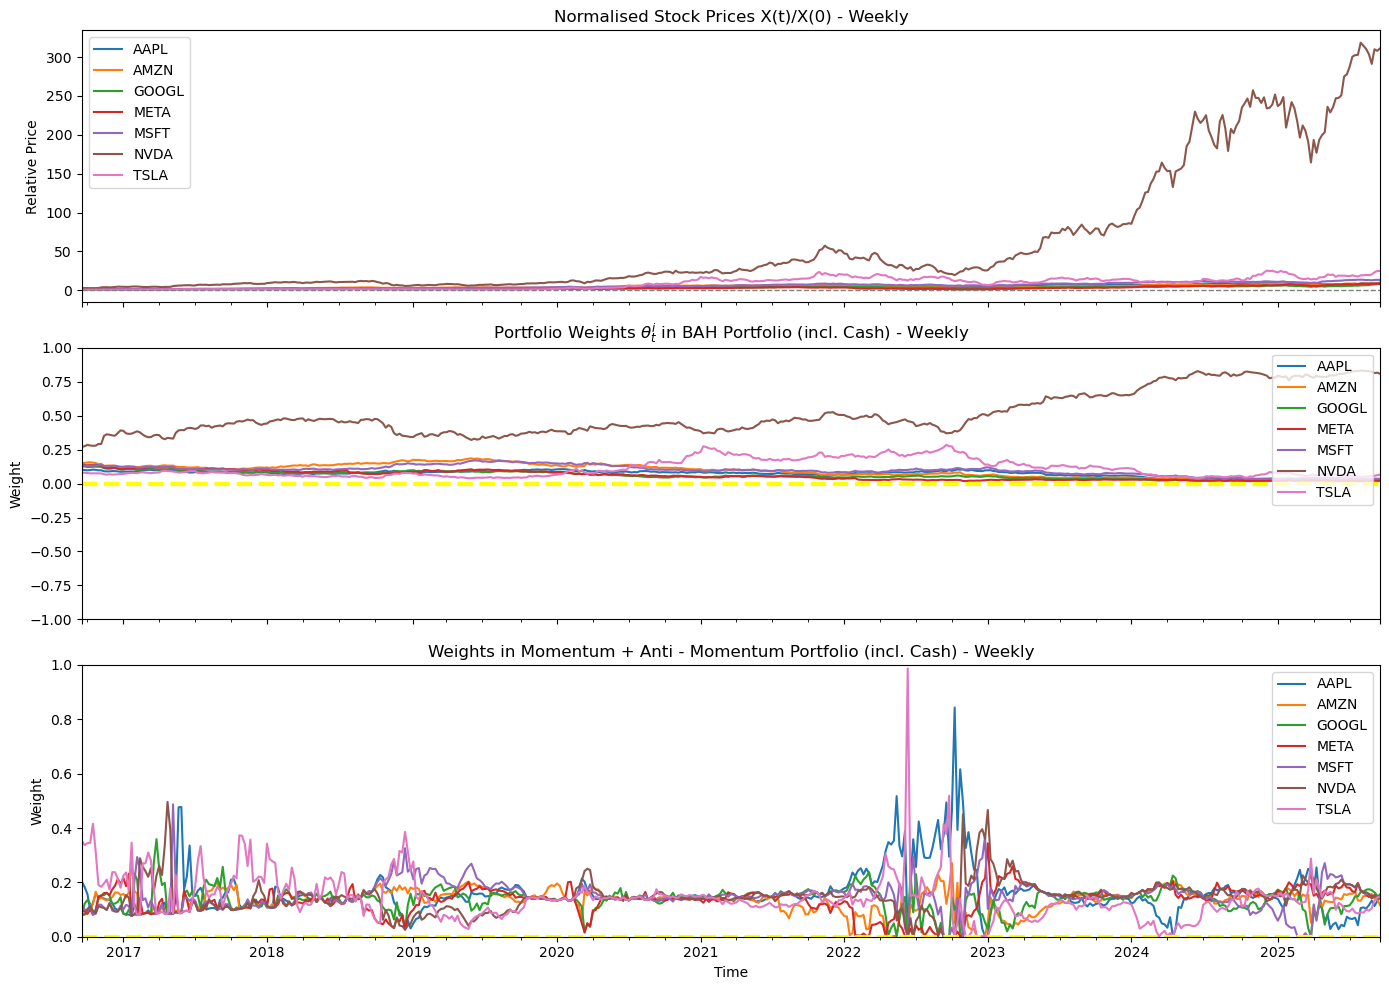
\includegraphics[width=0.95\textwidth]{Images/best_weekly_weights.png}
    \caption{Evolution of BAH and M+AM strategies in the “Magnificent Seven” universe. Top: Normalised asset prices show diverging performance, with \texttt{NVDA} driving exceptional cumulative gains. Middle: BAH portfolio weights become concentrated in top performers over time due to price appreciation, illustrating the strategy's inherent and growing exposure to individual winners. Bottom: M+AM dynamically reallocates based on signals, adapting to changing conditions but incurring turnover costs.}
    \label{fig:weights_best}
\end{figure}

Figure~\ref{fig:weights_worst} shows the evolution of the BAH and M+AM strategies for the ``Weakest Seven'' universe. The upper plot, showing normalised asset prices ($X_t/X_0$), visually confirms the secular decline of all assets, with some (e.g., \texttt{PARA}) effectively trending to zero. The middle panel depicts the market-capitalisation-like weights of the BAH portfolio under these conditions. Here, the only built-in risk buffer is mechanical: as an asset collapses, its portfolio weight shrinks accordingly. However, this adjustment lags reality and offers little real protection, since the capital was already lost during the decline.

The bottom panel, which traces the M+AM allocations, is more revealing. The strategy actively shifts its capital, at times concentrating heavily in a small number of relatively stronger assets, while avoiding the most severe decliners. This selective reallocation enabled M+AM to sidestep the deepest losses -- something unattainable for passive approaches like BAH or CRP. While the strategy is fully systematic and rule-driven rather than discretionary, it embodies an active allocation style: portfolio weights are recalibrated continuously in response to evolving price signals, leading to frequent reallocations and concentrated exposures.

\begin{figure}[htbp]
    \centering
    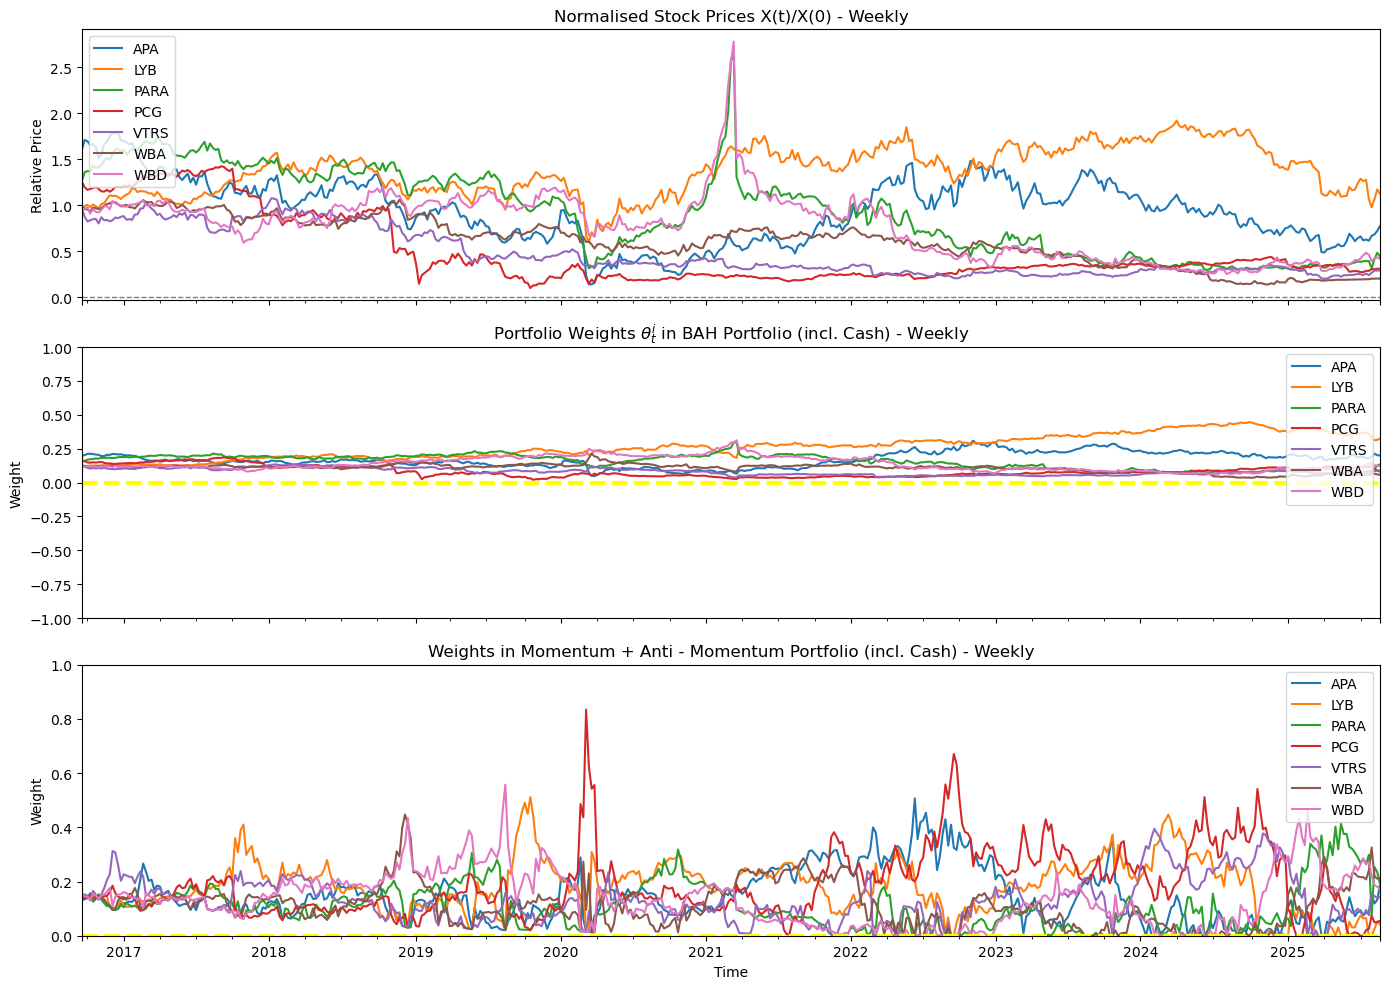
\includegraphics[width=0.95\textwidth]{Images/worst_weekly_weights.png}
    \caption{Portfolio composition analysis for the ``Weakest Seven''. Top: Normalised asset prices show universal decline. Middle: The evolving weights of the BAH strategy. Bottom: The active, concentrated allocations of the Momentum + Anti-Momentum strategy, which allowed for effective capital preservation.}
    \label{fig:weights_worst}
\end{figure}

\section{Summary of Weekly Allocation Results}

The weekly results underscore the critical role of regime dependence. In the high-growth ``Magnificent Seven'' regime, BAH delivered the highest terminal value and Sharpe ratio, but this success was driven by an increasingly concentrated bet on a few dominant winners like \texttt{NVDA}, which also resulted in the deepest drawdowns. CRP underperformed because its rebalancing rule systematically sold appreciating assets, limiting compounding. The M+AM strategy's aggressive rotations introduced high turnover and conflicting signals, preventing it from keeping pace. The Aggregated portfolio provided an effective compromise, achieving a Sharpe ratio competitive with BAH while offering meaningfully better drawdown protection through strategic diversification.

In the secular decline of the ``Worst Seven'' regime, all strategies suffered severe absolute losses. However, BAH and CRP performed worst in risk-adjusted terms (negative Sharpe ratios), as their passive, long-only rules offered no defence. The M+AM strategy's dynamic reallocations -- concentrating in relatively stronger assets and avoiding the worst decliners -- allowed it to achieve a marginally positive Sharpe ratio, though at the cost of elevated volatility and the largest single drawdown. The Aggregated portfolio again demonstrated resilience, delivering the most consistent performance across both regimes by dynamically blending its components.

These findings reinforce Cover’s universal portfolio intuition: concentration amplifies returns in booms but also magnifies risk, while adaptive strategies provide essential, though imperfect, protection in downturns. No single rule is optimal across all environments, but an ensemble approach that diversifies across these structural biases consistently avoids the worst outcomes and provides the most reliable long-term performance.

\chapter{Discussion and Conclusion}

The empirical investigation undertaken in this thesis evaluated five fundamental, hybrid portfolio allocation strategies -- Buy-and-Hold (BAH), Constantly Rebalanced Portfolio (CRP), Momentum, Anti-Momentum (Contrarian), and Aggregated strategies -- across two sharply contrasting market environments: the high-growth “Magnificent Seven” and a set of underperforming, structurally impaired equities. This dual-market analysis allowed for both stress testing and performance benchmarking across typical and adverse financial regimes. 

The results, analysed through the complementary measures of risk-adjusted returns (Sharpe ratio) and capital preservation (Maximal Drawdown), offer nuanced insights that both support and challenge established principles in the literature. This discussion interprets these findings, evaluates their alignment with existing research, and proposes directions for future work in an evolving financial landscape.

Importantly, these results are based on adjusted close prices, which strip out dividends, stock splits, and other corporate actions. This ensures that performance reflects true underlying price dynamics rather than mechanical distortions from payouts or structural events, allowing for clean comparisons across strategies.

The BAH strategy dominated in the high-growth “Magnificent Seven” portfolio, producing the highest terminal value and a relatively high Sharpe ratio (1.35). This aligns closely with the extensive evidence in favour of passive investing in sustained bull markets \citep{Siegel1998, Bogle1999}. Its strength came from allowing compounding to run without incurring trading costs, a classic advantage documented across multiple decades of equity performance. However, this came at the cost of severe downside exposure: its MDD exceeded –53\%, illustrating how fully passive allocations cannot shield against market-wide shocks such as the COVID-19 crash in 2020 or the 2022 inflation shock. Furthermore, the weight decomposition showed that BAH evolved into an extremely concentrated bet, with \texttt{NVDA} swelling to nearly 70\% of the portfolio. This phenomenon confirms Campbell and Viceira\textquotesingle s (\citeyear{Campbell2002}) warnings about “concentration drift” in passive allocations: portfolios diversified at inception can silently become dominated by a few outperformers, leaving investors exposed to idiosyncratic risk. The implication is that while BAH is unrivaled in growth environments, its Sharpe ratio masks the hidden fragility of concentration and large drawdowns.

The Constantly Rebalanced Portfolio (CRP) produced weaker outcomes. In the growth universe, its Sharpe ratio lagged BAH because continual rebalancing away from top performers curtailed compounding gains. Its MDD was somewhat lower (–47.9\%), but the improvement was marginal relative to the efficiency sacrificed. This result is consistent with \citet{Perold1988} and \citet{French2008}, who demonstrated that CRP systematically underperforms in trending markets by selling winners too early. In the declining universe, CRP failed even more dramatically: by reallocating into assets that continued to fall, it amplified losses and ended with the weakest performance overall. This echoes \citet{DeMiguel2009}, who showed that the benefits of frequent rebalancing are often illusory in the absence of mean reversion, and can be entirely offset once trading frictions are considered. Both its Sharpe ratio and MDD confirm the same lesson: CRP may succeed in volatile, mean-reverting environments \citep{Ilmanen2011}, but it is ill-suited to strong trends in either direction.

The M+AM strategy revealed a more complex picture. In the growth regime, it lagged with a lower Sharpe ratio than BAH, as high turnover and conflicting signals diluted its efficiency. Yet in the declining regime, it displayed resilience: by reallocating away from collapsing names, it achieved a marginally positive Sharpe ratio, standing in contrast to the negative outcomes of BAH and CRP. However, this advantage was offset by its MDD, which exceeded –70\% — the largest of all strategies. This paradox echoes \citet{Daniel2016} work on “momentum crashes”, where momentum-based rules can suddenly unravel during sharp reversals. The M+AM results therefore demonstrate both the promise and fragility of signal-driven approaches: they can sidestep average declines but remain acutely vulnerable to tail events. The weight analysis adds nuance: by shifting capital towards relatively “less weak” assets, the strategy avoided the universal decline seen in BAH, but the cost was heightened volatility and concentrated bets that left it exposed to rare but extreme losses.

In the stress-testing scenario, where portfolios were applied to weak or declining stocks, the distinctions between strategies became more pronounced. The Buy-and-Hold approach failed predictably, reflecting its structural inflexibility and sensitivity to poor asset selection. CRP exacerbated losses due to its insistence on reallocating into declining assets -- surprisingly increasing exposure to value traps and downward momentum. The most striking is M+AM’s combination of a marginally positive Sharpe ratio with the deepest drawdown in the “Worst Seven” universe. This suggests that risk-adjusted measures alone can obscure extreme vulnerabilities: investors may perceive stability on average while remaining exposed to catastrophic tail losses. The phenomenon mirrors the momentum crashes identified by \citet{Daniel2016} and suggests the need for additional downside protection overlays in signal-driven strategies. Similarly, CRP’s near-identical drawdowns to BAH in the declining regime raise questions about its protective value when mean reversion is absent, underscoring that rebalancing is not a universal safeguard.

The Aggregated strategy provided the most consistent outcomes across regimes. In growth markets, it achieved a Sharpe ratio close to BAH while lowering drawdown exposure (MDD –50.7\% compared to –53.9\% for BAH). In declining markets, it maintained a modest Sharpe advantage over BAH and CRP while containing drawdowns to levels comparable with M+AM. This supports Cover\textquotesingle s (\citeyear{Cover1991}) universal portfolio framework and subsequent evidence by \citet{Cover1996}): by diversifying not just across assets but across allocation rules, the Aggregated portfolio avoided catastrophic outcomes even when no single strategy succeeded outright. Its results also align with \citet{Fung2004}) and \citet{Ilmanen2011}, who emphasised the robustness of multi-strategy ensembles in hedge fund and asset allocation contexts. The Aggregated portfolio did not deliver the highest Sharpe in any single regime, but it consistently avoided being the worst, highlighting the practical value of diversification across investment philosophies.

Beyond empirical outcomes, this thesis contributes methodologically in several areas. Each strategy is articulated in terms of formal portfolio mappings, ensuring analytical clarity and consistency. The implementation includes realistic frictions via proportional fees and minimum execution costs, reflecting institutional trading conditions. The weekly rebalancing horizon avoids overfitting to high-frequency noise, and the rolling-window rationale in momentum strategies aligns with previous academic research \citep{Jegadeesh1993, Ilmanen2011}. Furthermore, the modular aggregation framework provides reusable simulation tools for multi-level portfolio nesting. These implementations form a foundation that can be extended to incorporate machine learning-based meta-strategies, regime-switching detection, or conditional rebalancing heuristics.

These findings also highlight avenues for future research. First, the analysis assumed frictionless execution, aside from excluding daily rebalancing due to its instability and implied costs. Incorporating realistic frictions — transaction costs, bid–ask spreads, slippage, and taxes — could significantly alter the viability of high-turnover strategies like M+AM and the Aggregated portfolio \citep{DeMiguel2009, vanVliet2016}. Second, the study’s design, contrasting extreme winners with extreme losers, provided a clear blueprint for regime testing but is not fully representative of diversified real-world portfolios. Extending the framework to balanced equity-bond or multi-asset allocations would provide broader insight into how these strategies perform under varied macroeconomic conditions, such as inflationary versus recessionary regimes \citep{Ilmanen2011}. Finally, regime detection remains the central challenge. Artificial Intelligence and machine learning offer promising avenues here: unsupervised learning, hidden Markov models or Bayesian approaches could identify prevailing regimes in real time, reinforcement learning could dynamically adjust the weighting of momentum and contrarian signals, and algorithmic execution could minimise transaction costs (see e.g., \citealp{Bryzgalova2023}).

In conclusion, this thesis demonstrates that portfolio strategy design is most robust when it incorporates multiple market hypotheses and adapts to shifting conditions. By analysing classical and behavioural strategies under both bullish and bearish asset universes, we confirm the inadequacy of static methods and the practical strength of strategic diversification. Aggregated portfolios, when constructed carefully, outperform not only in returns but in risk-resilience, especially as measured by Maximal Drawdown. The practical implication underscores the necessity of diversification that extends beyond asset classes to encompass the underlying investment philosophies themselves. Strategies that are overcommitted to a single market worldview -- whether it be efficiency, mean reversion, or trend persistence -- are inherently vulnerable to regime shifts and exhibit pronounced fragility when their core assumptions are invalidated. Strategy aggregation, framed and evaluated under drawdown risk, represents a promising path forward for investors seeking long-term growth without unacceptable capital erosion. Consequently, the future of portfolio allocation appears to lie in the development of adaptive systems, potentially enhanced by artificial intelligence, that can dynamically balance strategic biases to navigate complex and evolving financial markets.

\addcontentsline{toc}{chapter}{Bibliography}  
\bibliographystyle{agsm}   
\bibliography{reference}   

\appendix
\addcontentsline{toc}{part}{Appendices}
\titleformat{\chapter}[display]
  {\normalfont\bfseries\LARGE}
  {\appendixname\ \thechapter}{20pt}{\LARGE}
\chapter{Sensitivity Analysis of Rebalancing Frequencies}
\label{app:a}

This appendix presents a comprehensive sensitivity analysis of the portfolio strategies under daily and monthly rebalancing frequencies. The objective is to assess the robustness of the primary weekly results and to explore the performance limits at both extremes of the trading spectrum. The daily frequency tests the impact of high transaction costs and market microstructure noise, while the monthly frequency examines the consequences of potentially missing shorter-term trends due to slower reaction times.

% ==================== DAILY REBALANCING ====================
\section{Daily Rebalancing Frequency}
\label{app:a1}

\subsection{``Magnificent Seven'' Regime (Daily)}
\label{app:a1.1}

\begin{figure}[htbp]
    \centering
    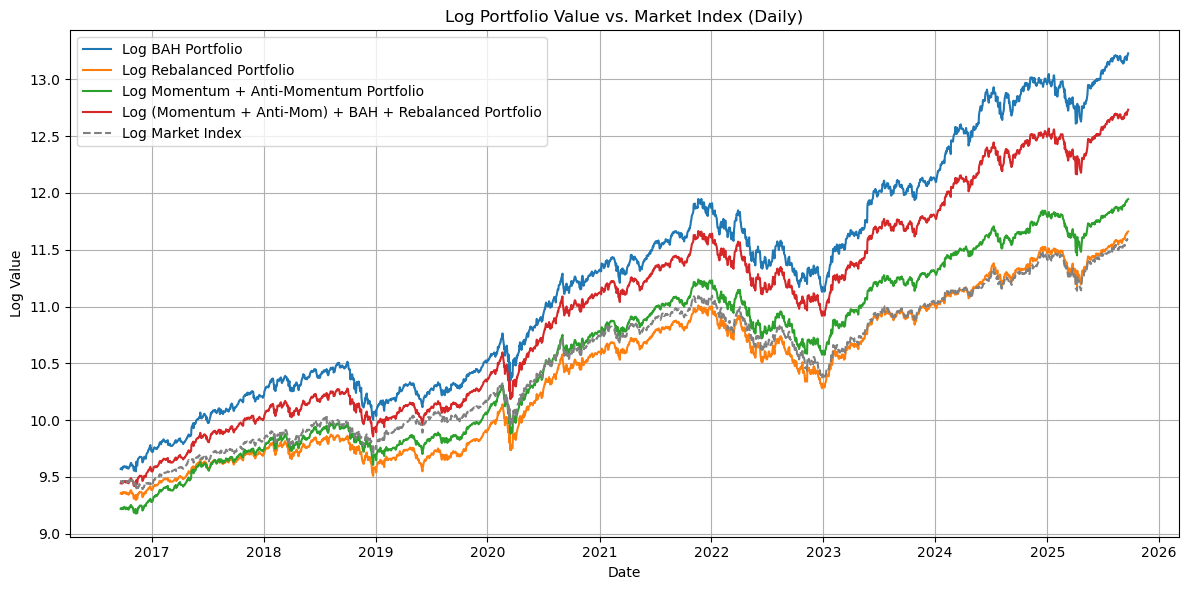
\includegraphics[width=0.95\textwidth]{Images/best_daily_log_values.png}
    \caption{Log Portfolio Value vs. Market Index (Daily) for the ``Magnificent Seven'' universe.}
    \label{fig:a1}
\end{figure}

\textbf{Figure A.1} illustrates the evolution of log portfolio values for the ``Magnificent Seven'' universe under daily rebalancing. In contrast to the smoother weekly trajectories, these daily paths exhibit significant high-frequency noise. Nonetheless, the relative performance hierarchy observed weekly is largely preserved: the BAH strategy achieves the highest terminal value, with the Aggregated portfolio tracking it closely. The paths of the M+AM and CRP strategies are notably more erratic.

The quantitative metrics in \textbf{Table A.1} provide a sharper perspective. Regarding capital preservation, the M+AM strategy registers the lowest maximal drawdown (MDD) of -48.48\%, indicating that daily signal updates can offer marginally better protection during sharp corrections compared to the weekly frequency. Conversely, the Aggregated portfolio's MDD (-52.62\%) aligns almost exactly with the market benchmark (-52.01\%). In terms of risk-adjusted returns, the Sharpe ratios tell a more critical story. While BAH (1.27) and the Aggregated portfolio (1.24) remain at the top, the absolute values for all strategies are lower than their weekly counterparts. Most strikingly, the CRP strategy's Sharpe ratio plummets to 0.99 (from 1.31 weekly), a clear indication of the severe impact of daily transaction costs on a high-turnover strategy.

\begin{table}[htbp]
    \centering
    \caption{Maximal Drawdown and Sharpe Ratio: ``Magnificent Seven'' (Daily)}
    \label{tab:a1}
    \begin{tabular}{lcc}
        \toprule
        Strategy & Maximal Drawdown & Sharpe Ratio \\
        \midrule
        BAH & -55.88\% & 1.27 \\
        CRP & -51.75\% & 0.99 \\
        M+AM & -48.48\% & 1.11 \\
        Aggregated & -52.62\% & 1.24 \\
        Market Index & -52.01\% & 0.99 \\
        \bottomrule
    \end{tabular}
\end{table}

\subsection{``Worst Seven'' Regime (Daily)}
\label{app:a1.2}

\begin{figure}[htbp]
    \centering
    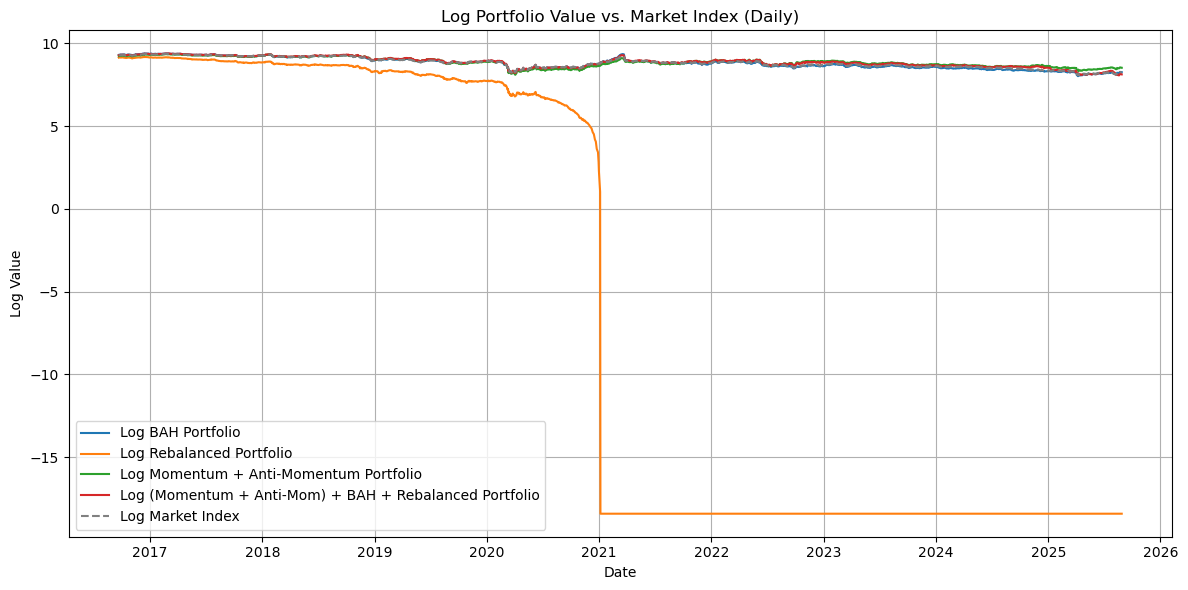
\includegraphics[width=0.95\textwidth]{Images/worst_daily_log_values.png}
    \caption{Log Portfolio Value vs. Market Index (Daily) for the ``Worst Seven'' universe.}
    \label{fig:a2}
\end{figure}

The results for the ``Worst Seven'' universe, shown in \textbf{Figure A.2}, reveal more severe implications. The log-value chart highlights the catastrophic performance of the CRP strategy, whose value trajectory collapses entirely. This visual finding is consistent with the extreme maximal drawdown of -166.13\% reported in \textbf{Table A.2}, suggesting total capital impairment. The other strategies mirror the dismal performance observed weekly, with the M+AM strategy showing no capacity for generating positive returns at this high frequency.

The risk-adjusted metrics in \textbf{Table A.2} further underscore the failure of active strategies in this stressed regime under daily trading. All Sharpe ratios are negative and generally worse than the weekly values. The CRP strategy's Sharpe ratio of -0.08, while less negative than BAH's -0.20, is a statistical artifact of its extreme volatility and failure rather than a sign of robustness. The Aggregated portfolio's Sharpe ratio of -0.26 is the poorest of all, demonstrating its inability to effectively synthesise its components under the noisy conditions of daily rebalancing in a bear market.

\begin{table}[htbp]
    \centering
    \caption{Maximal Drawdown and Sharpe Ratio: ``Worst Seven'' (Daily)}
    \label{tab:a2}
    \begin{tabular}{lcc}
        \toprule
        Strategy & Maximal Drawdown & Sharpe Ratio \\
        \midrule
        BAH & -74.83\% & -0.20 \\
        CRP & -166.13\% & -0.08 \\
        M+AM & -71.50\% & -0.12 \\
        Aggregated & -73.60\% & -0.26 \\
        Market Index & -72.89\% & -0.23 \\
        \bottomrule
    \end{tabular}
\end{table}

\subsection{Portfolio Weight Dynamics (Daily)}
\label{app:a1.3}

\begin{figure}[htbp]
    \centering
    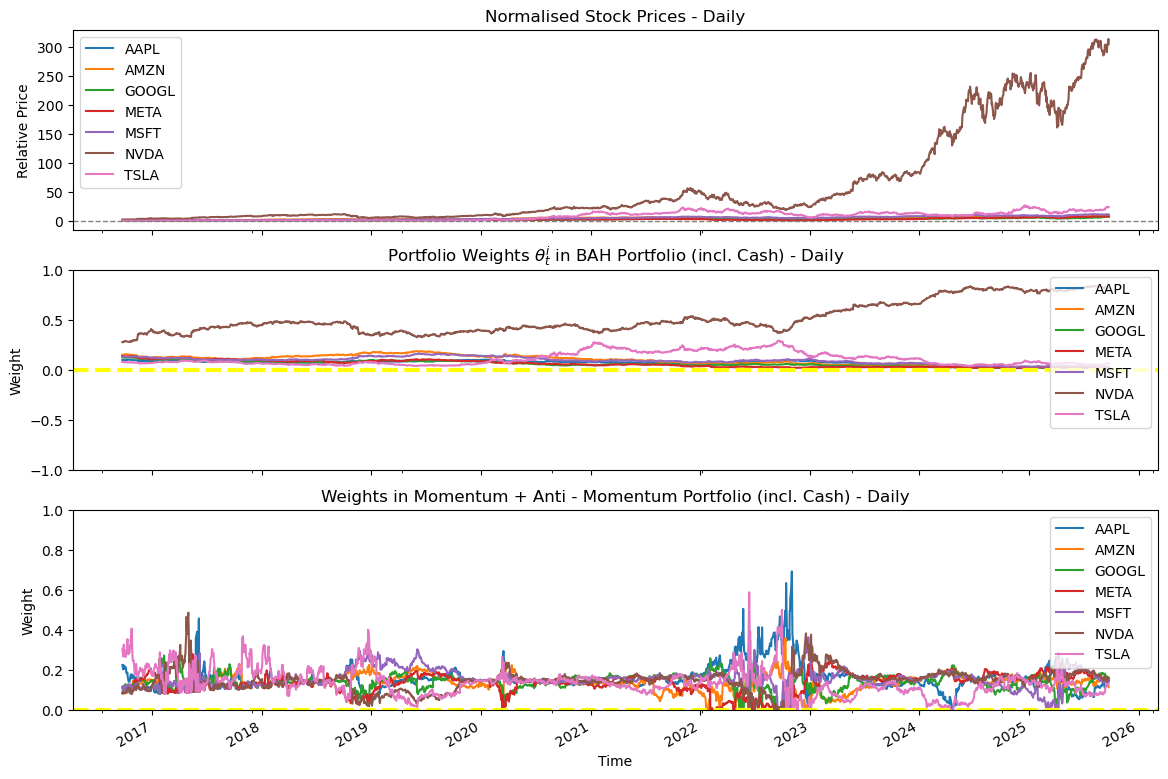
\includegraphics[width=0.95\textwidth]{Images/best_daily_weights.png}
    \caption{Portfolio weights for the ``Magnificent Seven'' (Daily).}
    \label{fig:a3}
\end{figure}

\begin{figure}[htbp]
    \centering
    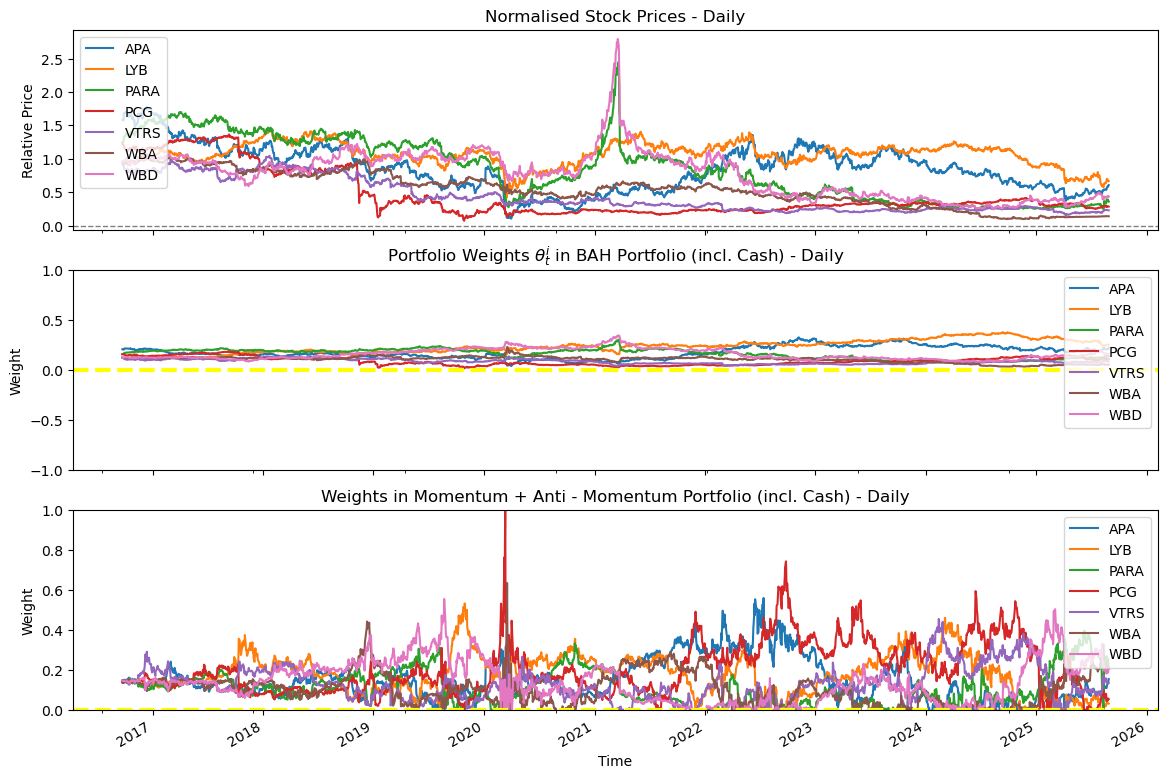
\includegraphics[width=0.95\textwidth]{Images/worst_daily_weights.png}
    \caption{Portfolio weights for the ``Worst Seven'' (Daily).}
    \label{fig:a4}
\end{figure}

The underlying mechanics of the strategies are illustrated in the weight evolution graphs. \textbf{Figure A.3} (``Magnificent Seven'') and \textbf{Figure A.4} (``Worst Seven'') display the portfolio allocations for the BAH and M+AM strategies. The BAH weights, while still reflecting the passive concentration in best performers like NVDA (Figure A.3) or the automatic reduction in collapsing assets like PARA (Figure A.4), are dominated by high-frequency jitter, obscuring the clear multi-week trends visible in the weekly analysis. For the M+AM strategy, the dynamic is even more pronounced. The allocations shift almost constantly, resulting in a chaotic and noisy profile. This indicates a strategy highly susceptible to market microstructure noise, leading to frequent, likely unprofitable, trades and implying impractically high turnover that would inevitably erode any theoretical returns through transaction costs. This visual evidence of frenetic trading directly corroborates the significantly degraded Sharpe ratios observed in the daily analysis.

\subsection{Conclusion for Daily Allocation}
\label{app:a1.4}

In summary, the analysis of daily rebalancing unequivocally demonstrates the practical limitations imposed by high transaction costs and market microstructure noise. The pronounced deterioration in Sharpe ratios for the CRP and M+AM strategies highlights that their theoretical benefits are negated by the costs of incessant trading, rendering them commercially unviable. This is visually corroborated by the frenetic, noisy reallocations observed in the weight graphs, which indicate counterproductive trading driven by short-term noise rather than meaningful signals. Consequently, the overall poor and unstable performance at the daily frequency strongly supports the selection of the weekly rebalancing interval as a more realistic and implementable benchmark for evaluating portfolio allocation strategies.

% ==================== MONTHLY REBALANCING ====================
\section{Monthly Rebalancing Frequency}
\label{app:a2}

\subsection{``Magnificent Seven'' Regime (Monthly)}
\label{app:a2.1}

\begin{figure}[htbp]
    \centering
    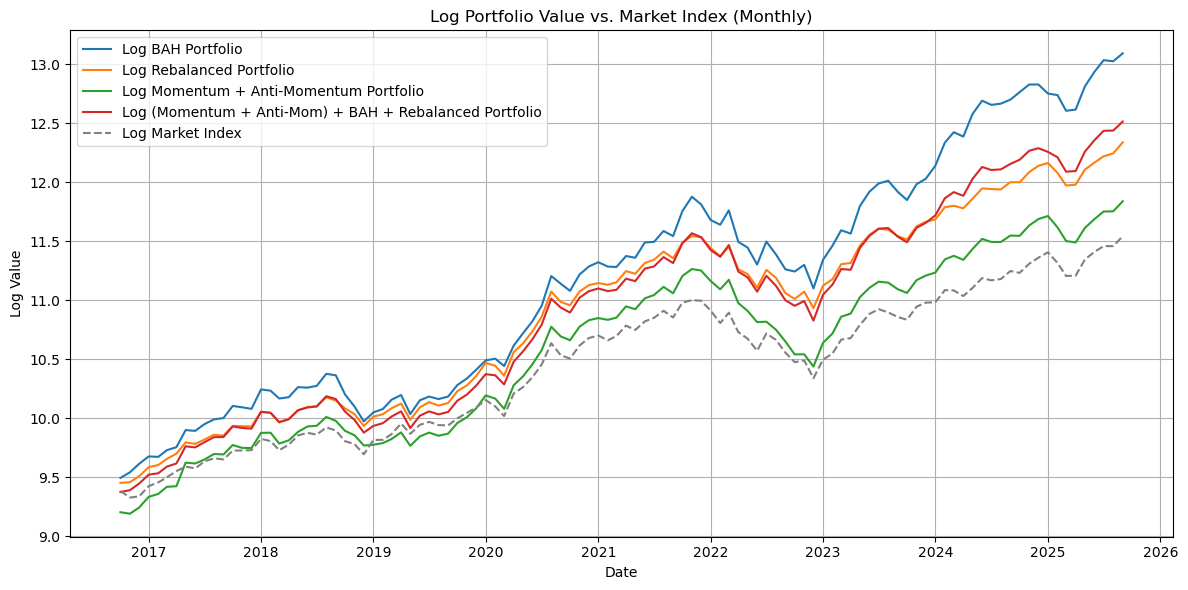
\includegraphics[width=0.95\textwidth]{Images/best_monthly_log_values.png}
    \caption{Log Portfolio Value vs. Market Index (Monthly) for the ``Magnificent Seven'' universe.}
    \label{fig:a5}
\end{figure}

\textbf{Figure A.5} displays the log portfolio values for the ``Magnificent Seven'' universe with monthly rebalancing. The trajectories are noticeably smoother than both the daily and weekly versions, with reduced high-frequency noise. The BAH strategy again shows strong performance, but the gap between it and the other strategies appears narrower than under weekly rebalancing.

The metrics in \textbf{Table A.3} reveal a notable shift in strategy hierarchy. The CRP strategy achieves the best MDD (-45.79\%) and the highest Sharpe ratio (1.34) in this regime. This indicates that monthly intervals are optimal for CRP's volatility harvesting mechanism, allowing trends to partially develop before triggering a rebalancing trade, thereby improving its risk-adjusted efficiency. The Aggregated portfolio remains competitive (Sharpe: 1.31), while the M+AM strategy lags with the worst drawdown (-56.23\%) and a lower Sharpe ratio (1.15), suggesting its signals are too stale when updated only monthly.

\begin{table}[htbp]
    \centering
    \caption{Maximal Drawdown and Sharpe Ratio: ``Magnificent Seven'' (Monthly)}
    \label{tab:a3}
    \begin{tabular}{lcc}
        \toprule
        Strategy & Maximal Drawdown & Sharpe Ratio \\
        \midrule
        BAH & -54.02\% & 1.33 \\
        CRP & -45.79\% & 1.34 \\
        M+AM & -56.23\% & 1.15 \\
        Aggregated & -52.29\% & 1.31 \\
        Market Index & -48.41\% & 1.08 \\
        \bottomrule
    \end{tabular}
\end{table}

\subsection{``Worst Seven'' Regime (Monthly)}
\label{app:a2.2}

\begin{figure}[htbp]
    \centering
    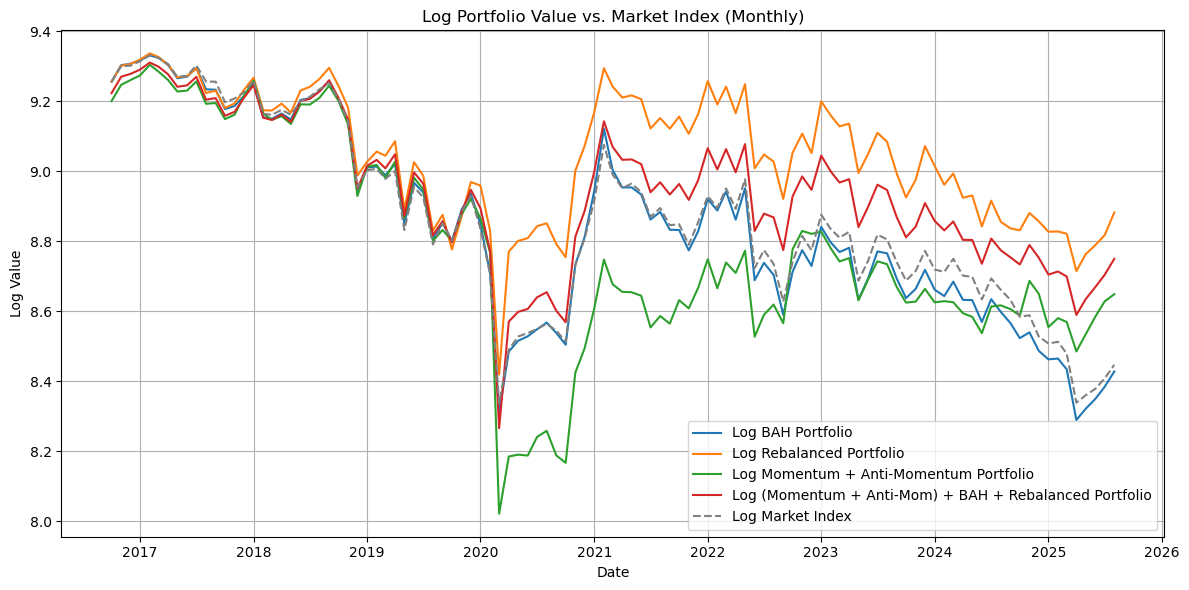
\includegraphics[width=0.95\textwidth]{Images/worst_monthly_log_values.png}
    \caption{Log Portfolio Value vs. Market Index (Monthly) for the ``Worst Seven'' universe.}
    \label{fig:a6}
\end{figure}

\textbf{Figure A.6} shows the log portfolio values for the ``Worst Seven'' universe. The monthly frequency does little to alter the dismal overall performance, with all strategies trending downward. However, the CRP strategy now performs marginally better relative to the others, no longer exhibiting the catastrophic failure seen in the daily frequency.

The data in \textbf{Table A.4} confirms this relative improvement for CRP, which registers the lowest MDD (-60.04\%) in this regime. The M+AM strategy, in contrast, performs the worst in terms of drawdown (-72.25\%), indicating that its reactive signals are ineffective when applied with a monthly lag in a rapidly declining market. The performances of BAH and the Aggregated portfolio are largely in line with the market benchmark.

\begin{table}[htbp]
    \centering
    \caption{Maximal Drawdown and Sharpe Ratio: ``Worst Seven'' (Monthly)}
    \label{tab:a4}
    \begin{tabular}{lcc}
        \toprule
        Strategy & Maximal Drawdown & Sharpe Ratio \\
        \midrule
        BAH & -64.69\% & -0.08 \\
        CRP & -60.04\% & -0.07 \\
        M+AM & -72.25\% & -0.12 \\
        Aggregated & -64.80\% & -0.10 \\
        Market Index & -63.00\% & -0.11 \\
        \bottomrule
    \end{tabular}
\end{table}

\subsection{Portfolio Weight Dynamics (Monthly)}
\label{app:a2.3}

\begin{figure}[htbp]
    \centering
    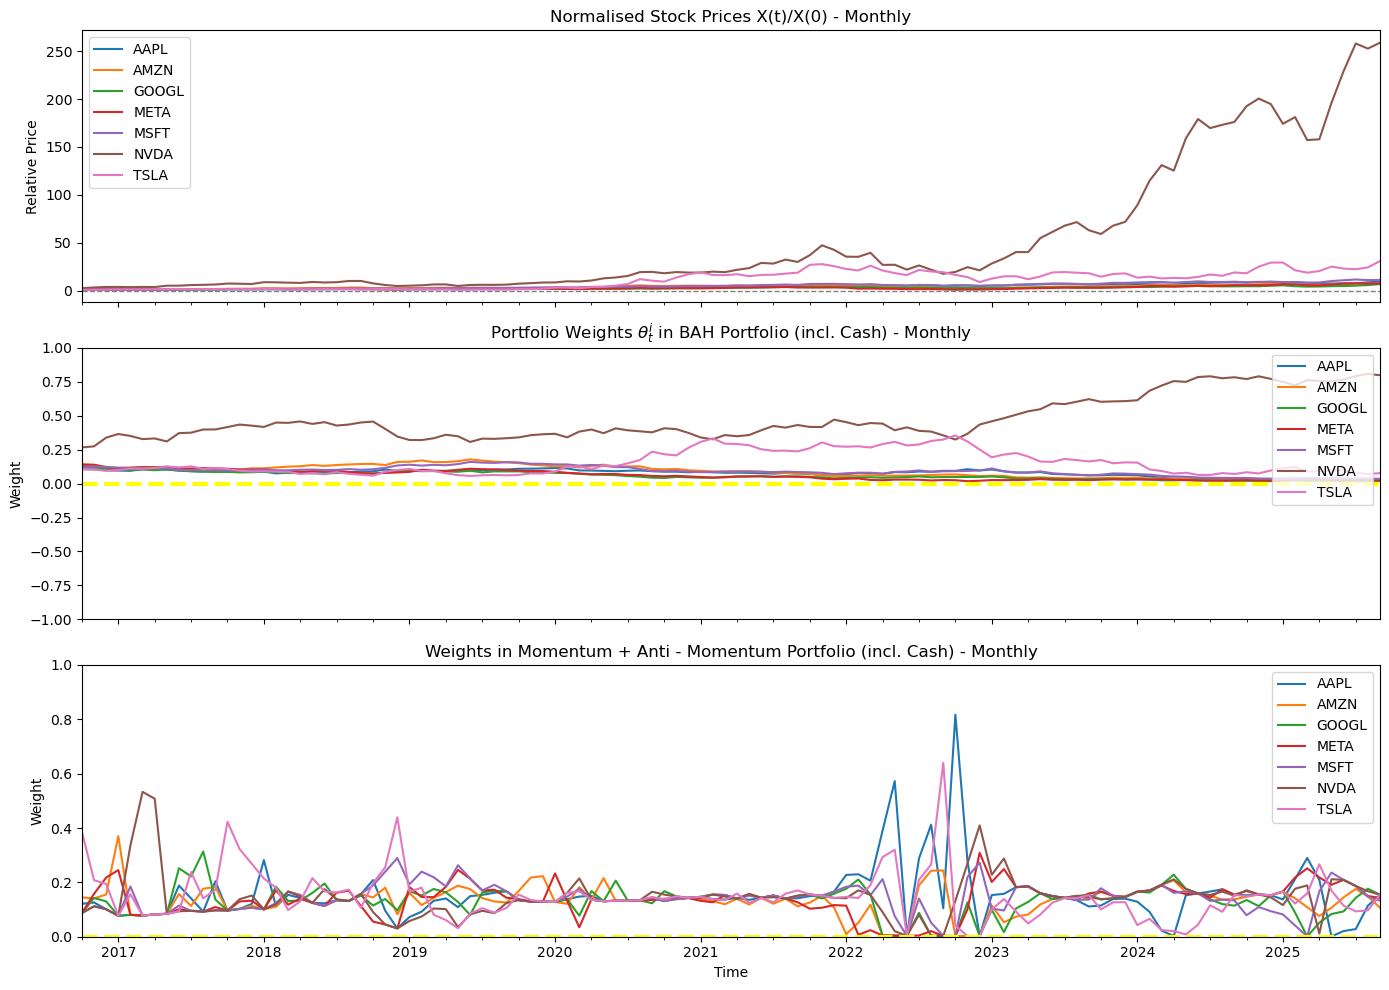
\includegraphics[width=0.95\textwidth]{Images/best_monthly_weights.png}
    \caption{Portfolio weights for the ``Magnificent Seven'' (Monthly).}
    \label{fig:a7}
\end{figure}

\begin{figure}[htbp]
    \centering
    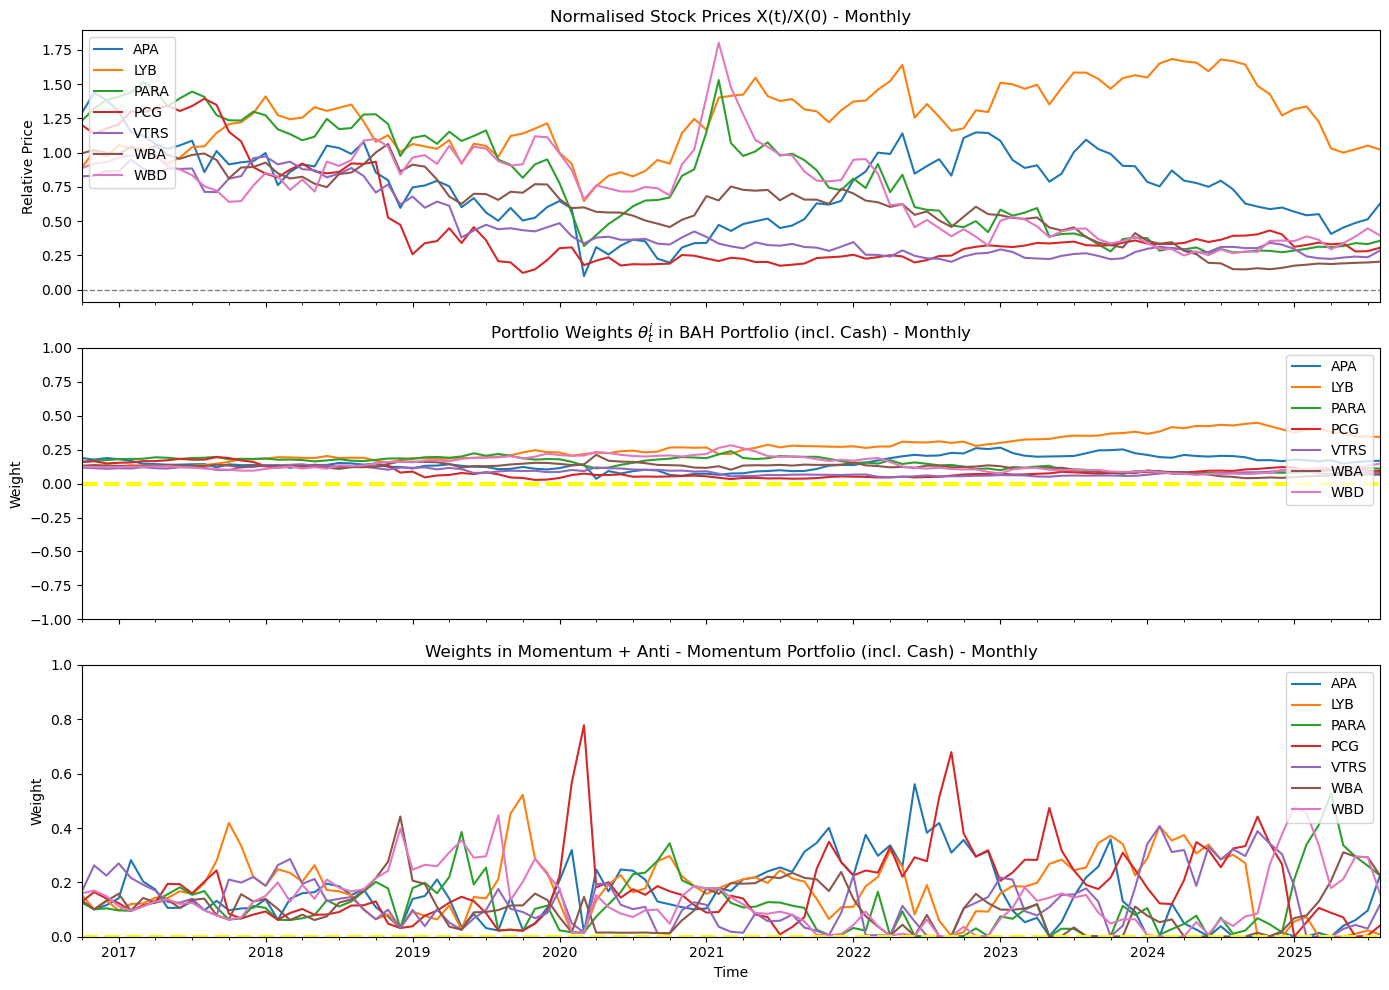
\includegraphics[width=0.95\textwidth]{Images/worst_monthly_weights.png}
    \caption{Portfolio weights for the ``Worst Seven'' (Monthly).}
    \label{fig:a8}
\end{figure}

\textbf{Figure A.7} (``Magnificent Seven'') and \textbf{Figure A.8} (``Worst Seven'') illustrate the portfolio allocations. The weight graphs are characterised by large, discrete steps, reflecting the monthly rebalancing intervals. The M+AM strategy's allocations appear sluggish and slow to react compared to the weekly charts, often holding positions for multiple months even as conditions change. The BAH strategy's passive concentration is, as expected, unaffected by the frequency.

\subsection{Conclusion for Monthly Allocation}
\label{app:a2.4}

The monthly rebalancing frequency provides contrasting insights, revealing a trade-off between turnover reduction and strategic responsiveness. This interval proves optimal for the CRP strategy, allowing trends to develop sufficiently for effective volatility harvesting without incurring excessive costs, thus maximising its risk-adjusted returns in the growth regime. Conversely, the infrequent rebalancing cripples the effectiveness of the M+AM strategy, whose signals become stale and lead to poor timing and amplified drawdowns. Therefore, while monthly rebalancing benefits specific strategies like CRP, it is detrimental to others, indicating that no single frequency is optimal for all approaches.

% ==================== COMPARATIVE CONCLUSION ====================
\section{Comparative Conclusion: Daily and Monthly vs. Weekly Sampling}
\label{app:a3}

The sensitivity analysis across daily and monthly frequencies ultimately reinforces the weekly horizon as the most robust and balanced choice for the multi-strategy framework of this thesis. The daily frequency is invalidated by prohibitive costs and noise, while the monthly frequency, though beneficial for CRP, is too sluggish for the momentum-based components. The weekly sampling effectively serves as a compromise, mitigating the costs that affect daily trading while preserving the responsiveness that monthly intervals lack. This balanced nature of the weekly frequency is crucial for the Aggregated portfolio, which relies on the timely interaction of its diverse components. Thus, the underperformance at both the daily and monthly extremes validates the weekly rebalancing not just as a convenient choice, but as the most appropriate temporal scale for implementing the strategic diversification that is central to this study.

\chapter{Implementation Code for Weekly Frequency Analysis}
\label{app:b}

This appendix provides the complete Python implementation used to generate the results for the weekly rebalancing frequency presented in the main analysis. The code is structured to analyse both the ``Magnificent Seven'' and ``Worst Seven'' portfolios, with the active portfolio selection controlled by commenting/uncommenting the respective ticker lists. The implementation includes strategy classes for Buy-and-Hold (BAH), Constant Rebalancing (CRP), Momentum, Anti-Momentum, and their aggregation, along with performance metric calculations and visualisation routines. The code is identical for the daily and monthly frequency allocations, the only difference being the interval specification in \texttt{yf.download} command (i.e., \texttt{"1d"}, \texttt{"1mo"}).

\begin{lstlisting}[language=Python, caption={Python implementation for weekly portfolio allocation analysis}, label=code:weekly_analysis, basicstyle=\footnotesize\ttfamily, breaklines=true, numbers=left]
import yfinance as yf
import numpy as np
import pandas as pd
import matplotlib.pyplot as plt

# === Parameters ===
# Tickers are stock data indices
tickers = ["AAPL", "MSFT", "NVDA", "AMZN", "META", "GOOGL", "TSLA"]  # Magnificent Seven
#tickers = ["WBD", "PARA", "APA", "WBA", "PCG", "VTRS", "LYB"]       # Worst Seven
equal_weight = 1 / len(tickers)
V0 = 10000 # Initial portfolio investment

# === Download data, normalise and compute returns  ===
data = yf.download(tickers, period="10y", interval="1wk", auto_adjust=False)["Adj Close"] # Historical data
data = data.dropna()  # Drop rows with missing data
weekly_returns = data.pct_change().dropna() # Compute weekly returns
normalized = data / data.iloc[0] # Normalise prices for BAH portfolio weights

# === Create series of theta values for BAH portfolio  ===
theta = normalized.shift(1).div(normalized.shift(1).sum(axis=1), axis=0)
# === Create series of equal weights for rebalanced portfolio  ===
crp_weights = np.array([equal_weight] * len(tickers))

# === Base Strategy Classes ===
class BuyAndHoldStrategy:
    def __init__(self, data, V0):
        self.data = data  # Historical price data
        self.V0 = V0      # Initial investment amount

    def run(self):
        # Normalise prices to initial values
        normalized = self.data / self.data.iloc[0]
        # Calculate portfolio value with equal initial weights
        values = (normalized * equal_weight).sum(axis=1) * self.V0
        # Calculate historical weight evolution
        weights = normalized.shift(1).div(normalized.shift(1).sum(axis=1), axis=0)
        return values, weights.fillna(0)

class ConstantRebalancedStrategy:
    def __init__(self, data, returns, crp_weights, V0, tc_rate=0.001):
        self.data = data                # Historical price data
        self.returns = returns          # Daily returns data
        self.crp_weights = crp_weights  # Equal weights for CRP
        self.V0 = V0                    # Initial investment amount
        self.tc_rate = tc_rate          # Transaction cost rate

    def run(self):
        values = [self.V0]
        n_assets = len(self.crp_weights)
        
        # Store weights at each time step
        weights_history = [self.crp_weights.copy()]
        
        # Start with target weights
        current_weights = np.array(self.crp_weights)
        current_values = self.V0 * current_weights
        
        for t in range(1, len(self.data)):
            # Calculate new asset values after price changes
            new_values = current_values * (1 + self.returns.iloc[t-1].values)
            portfolio_value_before = np.sum(new_values)
            
            # Calculate target values after rebalancing
            target_values = self.crp_weights * portfolio_value_before
            
            # Calculate trades needed (Δ_t^i)
            trades = target_values - new_values
            
            # Calculate transaction costs 
            transaction_costs = 0
            for trade in trades:
                if abs(trade) > 0:
                    # max(0.001 * |Δ_t^i|, 1)
                    cost_i = max(self.tc_rate * abs(trade), 1)
                    transaction_costs += cost_i
            
            # Apply transaction costs
            portfolio_value_after = portfolio_value_before - transaction_costs
            
            # Update current values with the new target values (adjusted for costs)
            current_values = target_values * (portfolio_value_after / portfolio_value_before)
            
            values.append(portfolio_value_after)
            weights_history.append(self.crp_weights.copy())  # Target weights remain constant
        
        # Create a DataFrame for weights with the same index as data
        weights_df = pd.DataFrame(
            weights_history, 
            index=self.data.index,
            columns=self.data.columns
        )
        
        return pd.Series(values, index=self.data.index), weights_df

class MomentumStrategy:
    def __init__(self, data, returns, lookback=52, tc_rate=0.001):
        self.data = data          # Historical price data
        self.returns = returns    # Daily returns data
        self.lookback = lookback  # Lookback period for momentum calculation
        self.tc_rate = tc_rate    # Transaction cost rate

    def run(self):
        # Calculate momentum signal using min-max normalisation
        roll_min = self.data.rolling(self.lookback).min()
        roll_max = self.data.rolling(self.lookback).max()
        momentum = (self.data - roll_min) / (roll_max - roll_min)
        
        # Calculate momentum weights (theta equivalent)
        theta_momentum = momentum.div(momentum.sum(axis=1), axis=0).fillna(0)

        values = [V0]
        transaction_costs = [0]

        for t in range(1, len(self.data)):
            if t < self.lookback:
                # Start trade with values from the previous allocation
                values.append(values[-1])
                transaction_costs.append(transaction_costs[-1])
                continue

            V_prev = values[-1]
            price_ratio = self.data.iloc[t] / self.data.iloc[t - 1]

            # Calculate trades needed and associated costs
            delta = (theta_momentum.iloc[t] * V_prev) - (theta_momentum.iloc[t - 1] * V_prev * price_ratio)
            cost = delta.abs().apply(lambda x: max(x * self.tc_rate, 1) if x > 0 else 0).sum()

            # Calculate portfolio growth from asset returns
            growth = np.dot(theta_momentum.iloc[t], self.returns.iloc[t - 1])
            V_new = (V_prev - cost) * (1 + growth)

            values.append(V_new)
            transaction_costs.append(transaction_costs[-1] + cost)

        return pd.Series(values, index=self.data.index), theta_momentum

class AntiMomentumStrategy:
    def __init__(self, data, returns, lookback=52, tc_rate=0.001):
        self.data = data
        self.returns = returns
        self.lookback = lookback
        self.tc_rate = tc_rate

    def run(self):
        roll_min = self.data.rolling(self.lookback).min()
        roll_max = self.data.rolling(self.lookback).max()
        anti_momentum = (roll_max - self.data) / (roll_max - roll_min)
        theta_anti_momentum = anti_momentum.div(anti_momentum.sum(axis=1), axis=0).fillna(0)

        values = [V0]
        transaction_costs = [0]

        for t in range(1, len(self.data)):
            if t < self.lookback:
                values.append(values[-1])
                transaction_costs.append(transaction_costs[-1])
                continue

            V_prev = values[-1]
            price_ratio = self.data.iloc[t] / self.data.iloc[t - 1]

            delta = (theta_anti_momentum.iloc[t] * V_prev) - (theta_anti_momentum.iloc[t - 1] * V_prev * price_ratio)
            cost = delta.abs().apply(lambda x: max(x * self.tc_rate, 1) if x > 0 else 0).sum()

            growth = np.dot(theta_anti_momentum.iloc[t], self.returns.iloc[t - 1])
            V_new = (V_prev - cost) * (1 + growth)

            values.append(V_new)
            transaction_costs.append(transaction_costs[-1] + cost)

        return pd.Series(values, index=self.data.index), theta_anti_momentum

# === Aggregator Class ===
class StrategyAggregator:
    def __init__(self, strategies):
        self.strategies = strategies  # List of strategy objects to aggregate

    def aggregate(self):
        weights_list = []  # Store weights from each strategy
        values_list = []   # Store values from each strategy

        # Run each strategy and collect results
        for strategy in self.strategies:
            V, w = strategy.run()
            values_list.append(V)
            weights_list.append(w)

        # Combine results into DataFrames/arrays for processing
        values_df = pd.concat(values_list, axis=1)
        weights_stack = np.stack([w.values for w in weights_list])
        values_array = values_df.values

        # Calculate aggregated weights based on strategy performance
        agg_weights = []
        for t in range(len(values_df)):
            v_t = values_array[t, :]  # Current values of all strategies
            theta_t = weights_stack[:, t, :]  # Current weights of all strategies
            # Calculate value-weighted average of strategy weights
            numerator = np.dot(v_t, theta_t)
            denominator = np.sum(v_t)
            agg_weights.append(numerator / denominator if denominator != 0 else np.zeros_like(numerator))

        # Create DataFrame for aggregated weights
        agg_weights_df = pd.DataFrame(agg_weights, index=values_df.index, columns=self.strategies[0].data.columns)
        
        # Calculate aggregated portfolio value using weights and returns
        agg_value = (agg_weights_df.shift(1).fillna(0) * weekly_returns).sum(axis=1).add(1).cumprod() * V0

        return agg_value, agg_weights_df

# === Wrapper class that converts precomputed portfolio values and weights into a strategy object ===
class WrappedStrategy:
    def __init__(self, value_series, weight_df, data):
        self._values = value_series  # Precomputed portfolio values
        self._weights = weight_df    # Precomputed portfolio weights
        self.data = data             # Reference to original price data (for compatibility)

    def run(self):
        # Return precomputed values and weights without additional processing
        return self._values, self._weights

# === Instantiate and Run ===
bah = BuyAndHoldStrategy(data, V0)
rebal = ConstantRebalancedStrategy(data, weekly_returns, crp_weights, V0)
mom = MomentumStrategy(data, weekly_returns)
anti = AntiMomentumStrategy(data, weekly_returns)

# === Aggregate Momentum and Anti-Momentum
aggregator1 = StrategyAggregator([mom, anti])  
agg_value1, agg_weights1 = aggregator1.aggregate()

# === Aggregate Momentum + Anti-Momentum, BAH and Constantly Rebalanced
aggregator5 = StrategyAggregator([wrapped_agg1, bah, rebal]) 
agg_value5, agg_weights5 = aggregator5.aggregate()

# === Market Index ===
market_index = (data.sum(axis=1) / data.sum(axis=1).iloc[0]) * V0
#print(market_index.head())

# === PLOT 1: Log Portfolio Values ===
plt.figure(figsize=(12, 6))
plt.plot(np.log(bah.run()[0][52:]), label="Log BAH Portfolio")
plt.plot(np.log(rebal.run()[0][52:].clip(lower=1e-8)), label="Log Rebalanced Portfolio")
plt.plot(np.log(agg_value1)[52:], label="Log Momentum + Anti-Momentum Portfolio")
plt.plot(np.log(agg_value5[52:]), color = 'red', label="Log (Momentum + Anti-Mom) + BAH + Rebalanced Portfolio")
plt.plot(np.log(market_index[52:]), label="Log Market Index", linestyle="--", color="gray")
plt.legend()
plt.title("Log Portfolio Value vs. Market Index (Weekly)")
plt.xlabel("Date")
plt.ylabel("Log Value")
plt.grid(True)
plt.tight_layout()
plt.show()

# === PLOT 2: Plot of theta time series against individual stock prices ===

fig, (ax1, ax2, ax3) = plt.subplots(3, 1, figsize=(14, 10), sharex=True)

# Top plot: normalised stock prices
normalized[52:].plot(ax=ax1)
ax1.axhline(0, color='gray', linestyle='--', linewidth=1)  
ax1.set_title("Normalised Stock Prices X(t)/X(0) - Weekly")
ax1.set_ylabel("Relative Price")
ax1.legend(loc="upper left")

# Middle plot: theta values BAH + cash position
theta[52:].plot(ax=ax2)
ax2.axhline(0, color='yellow', linestyle='--', linewidth=3)  
ax2.set_title(r"Portfolio Weights $\theta_{t}^i$ in BAH Portfolio (incl. Cash) - Weekly")
ax2.set_ylabel("Weight")
ax2.set_ylim(-1, 1)
ax2.legend(loc="upper right")
ax2.set_xlabel("Time")

# Middle plot: momentum and anti-momentum weights + cash position
agg_weights1[52:].plot(ax=ax3)
ax3.axhline(0, color='yellow', linestyle='--', linewidth=3)  
ax3.set_title(r"Weights in Momentum + Anti - Momentum Portfolio (incl. Cash) - Weekly")
ax3.set_ylabel("Weight")
ax3.set_ylim(0, 1)
ax3.legend(loc="upper right")
ax3.set_xlabel("Time")

plt.tight_layout()
plt.show()

# === Compute MDD (maximal drawdown) ===
def compute_max_drawdown(series):
    running_max = series.cummax()
    drawdown = (series - running_max) / running_max
    max_drawdown = drawdown.min()
    return max_drawdown

# === Compute MDD of each portfolio ===
mdd_bah = compute_max_drawdown(bah.run()[0])
mdd_rebalanced = compute_max_drawdown(rebal.run()[0])
mdd_momentum = compute_max_drawdown(agg_value1)
mdd_aggregated = compute_max_drawdown(agg_value5)
mdd_market = compute_max_drawdown(market_index)

print(f"Max Drawdown (BAH):                {mdd_bah:.2%}")
print(f"Max Drawdown (Rebalanced):         {mdd_rebalanced:.2%}")
print(f"Max Drawdown (Momentum):           {mdd_momentum:.2%}")
print(f"Max Drawdown (Aggregated):         {mdd_aggregated:.2%}")
print(f"Max Drawdown (Market):             {mdd_market:.2%}")

# === Compute Sharpe Ratio ===
def compute_sharpe_ratio(portfolio_values, risk_free_rate=0.0, freq_per_year=52, annualize=True):
    returns = portfolio_values.pct_change().dropna()

    # Convert annual risk-free rate to per-period rate
    rf_per_period = (1 + risk_free_rate) ** (1 / freq_per_year) - 1

    # Excess returns
    excess_returns = returns - rf_per_period

    # Sharpe ratio (non-annualised)
    sharpe = excess_returns.mean() / excess_returns.std()

    if annualize:
        sharpe *= np.sqrt(freq_per_year)

    return sharpe

# === Compute Sharpe Ratio of each portfolio ===
sharpe_bah = compute_sharpe_ratio(bah.run()[0])
sharpe_rebalanced = compute_sharpe_ratio(rebal.run()[0])
sharpe_momentum = compute_sharpe_ratio(agg_value1)
sharpe_aggregated = compute_sharpe_ratio(agg_value5)
sharpe_market = compute_sharpe_ratio(market_index)

print(f"Sharpe Ratio (BAH):                                             {sharpe_bah:.2f}")
print(f"Sharpe Ratio (Rebalanced):                                 {sharpe_rebalanced:.2f}")
print(f"Sharpe Ratio (Momentum + Anti-Momentum):     {sharpe_momentum:.2f}")
print(f"Sharpe Ratio (Aggregated):                                  {sharpe_aggregated:.2f}")
print(f"Sharpe Ratio (Market):                                          {sharpe_market:.2f}")
\end{lstlisting}



% === References ===
%\bibliographystyle{agsm}  % Harvard style
%\bibliography{references} % Create references.bib separately

\end{document}